\documentclass[declaration,shortabstract,english,mgr,pdftex,dvipsnames]{iithesis}

\graphicspath{{img/}}

\usepackage{minted}
\usepackage{pifont}
\usepackage{listings}
\usepackage{enumitem}
\usepackage{indentfirst}
\usepackage{bytefield}
\usepackage{pgfplots}
\usepackage{caption}
\usepackage{subcaption}

\setlength{\parindent}{1em}
\setmintedinline{breaklines,breakafter=,}

\pgfplotsset{compat=newest}
\pgfplotsset{scaled x ticks=false, scaled y ticks=false}

\newcommand{\comment}[1]{{
  \it \noindent
  \color{purple}
  COMMENT: #1
}}

\newcommand{\pr}[2]{{\tt (\##1) #2}\footnote{\url{https://github.com/cahirwpz/mimiker/pull/#1}}}

% Arguments
% 1 - file with old
% 2 - file with new
% 3 - additional axis args
\newcommand{\createhist}[3]{
  \begin{tikzpicture}[font=\tiny, trim axis left, trim axis right]
    \begin{axis}[ybar, ymin=0, #3]
      \addplot +[hist={data=x, bins=100}, opacity=0.5, draw=none, gray] table [y index=0] {#1};
      \addplot +[hist={data=x, bins=100}, opacity=0.5, draw=none, blue] table [y index=0] {#2};
      \legend{
        Old -- \input|"wc -l #1 | cut -d' ' -f1" invocations,
        New -- \input|"wc -l #2 | cut -d' ' -f1" invocations
      }
    \end{axis}
  \end{tikzpicture}
}

\newcommand{\createbar}[2]{
  \begin{tikzpicture}[font=\tiny, trim axis left, trim axis right]
    \begin{axis}[
        xmin=0, xmax=3, xtick={1,2},
        x tick style={draw=none},
        xticklabels={Old,New},
        ymin=0,
        nodes near coords,
        every axis plot/.append style={
          ybar,
          bar width=1cm,
          bar shift=0pt,
          fill,
          text opacity=1, fill opacity=0.5,
        }
    ]
      \addplot[draw=none, fill=gray] coordinates {(1, #1)};
      \addplot[draw=none, fill=blue] coordinates {(2, #2)};
    \end{axis}
  \end{tikzpicture}
}


\author{Franciszek Zdobylak}
\transcriptnum{XXXXXX}
\advisor{
    Krystian Bacławski
  \fmlinebreak
    Piotr Witkowski
}

\englishtitle{Effective copy-on-write mechanism \fmlinebreak for the Mimiker kernel}
\polishtitle{Efektywny mechanizm copy-on-write \fmlinebreak dla systemu operacyjnego Mimiker}

\englishabstract{
  This thesis presents an implementation of the virtual memory subsystem in the Mimiker operating system.
  It was created to enable the implementation of an efficient copy-on-write mechanism.
  The described implementation is based on a solution called UVM derived from the NetBSD system.
  Improvements in operating system memory management are particularly important, since memory is one of the most important resources in
  computer systems.
  The performance of a system can be estimated by measuring two factors: the memory used and the time taken to execute individual functions.
  This work also presents a performance analysis of the implemented solution.
}

\polishabstract{
  Niniejsza praca przedstawia implementację systemu pamięci wirtualnej w systemie operacyjnym Mimiker.
  Została ona stworzona, aby umożliwić zaimplementowanie efektywnego mechanizmu copy-on-write.
  Opisana implemenatacja jest oparta na rozwiązaniu o nazwie UVM pochodzącym z systemu NetBSD.
  Usprawnienia w zakresie zarządzania pamięcią systemu operacyjnego są szczególnie ważne, ponieważ pamięć jest jednym z najważniejszych zasobów w
  systemach komputerowych.
  Wydajność systemu można oszacować mierząc dwa czynniki: użytą pamięć oraz czas wykonywania poszczególnych funkcji.
  W tej pracy jest również przedstawiona analiza wydajności zaimplementowanego rozwiązania.
}

\begin{document}
\chapter{Introduction}
\label{chapter:introduction}

Mimiker is a UNIX operating system inspired by systems from the BSD family.
It is used to teach about UNIX kernel design so it has to implement the most important mechanisms of such a kernel
while still being simple and possible to understand.
One of the most important part of the kernel is the {\it Virtual Memory subsystem (VM)},
which is responsible for managing memory available in the system and providing it to the processes started by users.
Virtual Memory subsystem consists of various mechanisms that effectively manage memory.

The main goal of this thesis is to implement a copy-on-write mechanism in Mimiker.
It is the mechanism which reduces the amount of memory used by processes and speeds up the creation of them.
To measure if that objectives are met I've also created a tool for measuring performance of the kernel.
Additionally, while working on the copy-on-write mechanism I have improved the overall implementation of Virtual Memory in Mimiker,
both in terms of performance and functionality.

In the rest of this chapter we will see how processes use the memory and what operations should be implemented by the operating system kernel.
Our implementation of VM should provide all these operations.\footnote{
  In fact some of the features described below are not implemented in Mimiker yet.
  They require improvements or new types of operations in subsystems other than the virtual memory.
  The work described in this thesis does not cover this, but the new implementation of the VM is ready
  to be extended with the missing features as soon as all the necessary kernel mechanisms are ready to support them.
}
The copy-on-write, as it is a optimization, should not change the semantics of those operations.

%\begin{itemize}
%  \item We have a basic implementation of VM in Mimiker.
%  \item Based on the implementation from FreeBSD
%  \item We want to keep the semantics of system calls (and improve it to match the POSIX specification)
%  \item We want to change only the internal implementation
%  \item We want to improve it:
%    \begin{itemize}
%      \item Save memory by sharing it between processes when it is possible (CoW)
%      \item Speed up fork
%      \item Simplify the implementation of VM to make it easier to extend with new features
%      \item Create a tool to verify if the new implementation performs well
%    \end{itemize}
%  \item To understand how
%\end{itemize}

\section{Process virtual memory}

In operating systems, which support virtual memory, each user processes has its own {\it virtual address space}.
The process has an illusion, that it has all memory available only to itself.
To maintain this abstraction, the OS kernel has to carefully allocate real (physical) memory to store processes' data.
The whole layout of the process virtual memory is described in a {\it virtual memory map}.
It also contains information how to find the real location of the process memory.

The memory of the process is logically divided into segments.
The {\it memory segment} is a contiguous part of the process memory which has the same attributes.
There are few attributes that can describe different segment types:
\begin{itemize}
  \item Access protection -- process might be able to perform only few operations on the memory (read, write or execute).
  \item Source of the memory -- memory may come from a file, device registered in the system or might be created without any data.
  \item Visibility -- segment might be private for the process or shared between multiple processes.
\end{itemize}

%For each user process, the kernel creates and manages a separate virtual address space.
%It creates a {\it virtual memory map} to describe all the memory used by the process.
%It consists of many segments which representing regions of memory with the same properties.
%The segments don't have to describe contiguous memory and usually there are regions of unmapped memory between used segments.
%
%Besides VM~map, each process has its own page table to store its mappings from virtual to physical addresses.
%MMU uses it to perform address translation when that process is running.
%
%These structures sometimes may be confused with each other while being used for different things.
%VM~map completely describes the memory of the process, and has always the most recent information about all memory segments.
%The page table keeps track of currently used pages and is updated over time with new and changed address mappings.
%This difference is most noticeable when the process starts.
%Its VM~map has entries that describe its code, data and stack, but page table is empty because there wasn't made any memory access yet.

\subsubsection{Typical memory map}

The user process in Mimiker OS usually has at least six typical memory segments.
The table~\ref{tab:vm_map} describes these segments with their address ranges and access permissions.
Programs in real operating systems often have more memory segments in their memory map
(e.g. the heap or segments containing shared libraries data).

In Mimiker, the layout of the memory map is deterministic.
The first segment starts at 0x400000, and the next segments are placed directly after the previous one
(except for sbrk and stack, which are placed at other hard-coded addresses).
In more advanced operating systems, the layout of the address space is randomized.
This makes it harder to predict the addresses that will be used during program execution
(it prevents some types of attacks on the running software).
This technique is called {\it address space layout randomization (ASLR)} \cite{tannenbaum}.

\begin{table}[b]
  \centering
  \begin{tabular}{|c|c|c|c|}
    \hline
    \mintinline{c}{segment} & \mintinline{c}{start}      & \mintinline{c}{end}       & \mintinline{c}{prot}         \\
    \hline
    \mintinline{c}{code}   & \mintinline{c}{0x400000}       & \mintinline{c}{0x42e000}       & \mintinline{c}{READ | EXEC}         \\
    \mintinline{c}{data}   & \mintinline{c}{0x42e000}       & \mintinline{c}{0x431000}       & \mintinline{c}{READ | WRITE}        \\
    \mintinline{c}{rodata} & \mintinline{c}{0x431000}       & \mintinline{c}{0x439000}       & \mintinline{c}{READ}                \\
    \mintinline{c}{bss}    & \mintinline{c}{0x439000}       & \mintinline{c}{0x43e000}       & \mintinline{c}{READ | WRITE}        \\
    \mintinline{c}{sbrk}   & \mintinline{c}{0x8000000}      & \mintinline{c}{0x8003000}      & \mintinline{c}{READ | WRITE}        \\
    \mintinline{c}{stack}  & \mintinline{c}{0x7fffff7f0000} & \mintinline{c}{0x7fffffff0000} & \mintinline{c}{READ | WRITE | EXEC} \\
    \hline
  \end{tabular}
  \caption{Typical process VM~map in the Mimiker OS}
  \label{tab:vm_map}
\end{table}

In addition, the process address space also contains the kernel memory (which is not visible in the process VM~map).
It is located at high addresses and is protected from any access by the user program.
The kernel code and data must be visible in any address space because the kernel must be able to operate in any context.
Therefore, during context switching, when the address space is replaced with another process address space,
the kernel portion of memory remains unchanged.

On the other hand, the kernel must be able to modify process memory.
When a process requests some action from the kernel (using a system call interface), it is usually associated
with data movement (either from user to kernel or vice versa).
For example, during the \mintinline{c}{read} and \mintinline{c}{write} system calls, the process provides a buffer that is located in its memory.
Then, the kernel reads the data from that buffer (and writes it to the file referenced by the file descriptor),
or writes the data fetched from the file to that buffer.

\subsection{Types of memory segments}

There are several types of memory segments that are used by the processes for different purposes.
They can be categorized by two attributes: the type of memory they represent,
and the way they are shared between multiple processes.

\begin{description}[style=nextline]
  \item[Memory mapped file segments]
    Such segments contain data from a file stored in the file system mounted in the OS.
    We can specify whether changes made to their memory should also be written to the file or not.
    Segments representing file memory may also be swapped out using the file system, if possible.

    (Resources other than files that are available in the operating system may also be visible as memory in the process's memory map.
    Normally, all resources in UNIX systems are represented as files, so this case can also be called a memory mapped file).

  \item[Anonymous memory segments]
    The anonymous segments do not contain data associated with any resource present in the OS.
    They are initially filled with zeros because there is no place to read their contents from.
    Such segments are always swapped out to the swap space on a disk.
    After such a segment is destroyed, its data is lost and is not written to any file or other resource.

  \item[Private memory segments]
    They are visible only to the process that owns them.
    This means that the process has a private copy of the memory represented by such segments.
    Any operations performed on it will only be noticed by that process and no other.

    In the case of a privately mapped file, its contents are read from the file system,
    but any modifications are made to the process' copy of it.
    Private segments are usually swapped out using swap space on disk
    (the only exception to this rule is a situation when the segment read from the file hasn't been modified yet).
    After they are destroyed, their memory isn't saved anywhere.

  \item[Shared memory segments]
    Shared segments represent memory that is shared by multiple processes.
    Memory may be shared directly between processes if the same segment is present in multiple memory maps.
    Such a configuration can be obtained by creating a fork of a process that has a memory segment marked as shared.

    The other way is to share memory through the file system.
    When a file is mapped to process memory as shared, all write operations to the memory are also reflected by the file system,
    making them visible to other processes.
    Only files can be shared this way.

\end{description}

Different types of segments are used for different tasks.
Mapping file into the process memory is a convenient way to make faster I/O operations. % XXX: Are you sure about it???
The anonymous segments can be used as an inter-process communication method.
The memory mapping details are described in 9.8 in \cite{csapp} or in the \mintinline{c}{mmap} system call manual \cite{man:freebsd}.

\subsection{System calls related to the process VM}

There are several operations that can modify the process memory map.
They fall into two categories:
\begin{itemize}
  \item Modify the VM~map directly: \mintinline{c}{mmap}, \mintinline{c}{munmap}, \mintinline{c}{mprotect}.
  \item Change the VM~map as a result of another action: \mintinline{c}{fork}, \mintinline{c}{execve}, \mintinline{c}{exit}.
\end{itemize}

Besides the above system calls there are other which operate on the process memory map.
The ones that I mention here are implemented in all UNIX systems, also in Mimiker OS,
because they provide basic functionality needed to manage process virtual memory.

\begin{description}[style=nextline]
  \item[\mintinline{c}{void *mmap(void address, size_t len, int prot, int flags, int fd, off_t offset);}]
    The \mintinline{c}{mmap} function is used to allocate a new memory segment  of the specified size (\mintinline{c}{lenght}).

    The \mintinline{c}{address} argument is used as a hint for the kernel, where to place the created mapping in the process's
    memory map.
    If this is impossible, the kernel will choose another location for the new segment.
    This behavior might be modified by \mintinline{c}{MAP_FIXED} flag which tells the kernel that the location of the new segment
    must exactly as specified.
    Additionally, by adding one more flag (\mintinline{c}{MAP_EXCL}) we could ask kernel to fail if there exists
    any mapping within requested range.

    The \mintinline{c}{prot} argument specifies the types of memory operations that will be possible on the new memory
    (\mintinline{c}{PROT_EXEC}, \mintinline{c}{PROT_READ}, \mintinline{c}{PROT_WRITE}, \mintinline{c}{PROT_NONE}).

    The \mintinline{c}{flags} arguments determine the type of segment and specify the detailed behavior of the \mintinline{c}{mmap} function
    (\mintinline{c}{MAP_SHARED}, \mintinline{c}{MAP_PRIVATE}, \mintinline{c}{MAP_ANONYMOUS}, \mintinline{c}{MAP_EXCL}).

    The \mintinline{c}{fd} and \mintinline{c}{offset} arguments are used to specify the file and the offset in the file,
    where the mapping will begin.

  \item[\mintinline{c}{int munmap(void address, size_t length);}]
    \mintinline{c}{munmap} function is used to free the specified fragment of the memory (determined using the starting
    \mintinline{c}{address} and the \mintinline{c}{length}).
    The released memory doesn't have to to be represented by a single segment
    (e.g. it can belong to two adjacent segments) or to have the same properties.

  \item[\mintinline{c}{int mprotect(void addr, size_t len, int prot);}]
    The \mintinline{c}{mprotect} system call is used to change the access protection of the existing memory region.
    The modified memory region doesn't have to be within a single segment (similar to \mintinline{c}{munmap}).

    The protection is only changed in the memory map of the process that called \mintinline{c}{mprotect}.
    Each process sharing the segment affected by this call uses its own protection flags
    (so one process may have mapped the segment as read-only,
    but the other may write to the memory described by that segment).

  \item[\mintinline{c}{pid_t fork(void);}]
    \mintinline{c}{fork} creates an identical copy of the calling process.
    The new process is called a {\it child}, while the original is a {\it parent}.
    If \mintinline{c}{fork} succeeds, it returns twice (in the parent with the pid of the child and in the child with the value of 0).

    The child's VM~map is identical to the parent's VM map.
    Each private memory segment must be copied, and the shared memory is now also shared between the parent and the child.

  \item[\mintinline{c}{int execve(const char *pathname, char *argv[], char *envp[]);}]
    \mintinline{c}{execve} is used to start the execution of a new binary, without creating a new process.
    Combined with \mintinline{c}{fork}, these two operations are used to start new programs.

    The path to the binary file is specified with \mintinline{c}{pathname}.
    The new process is started with the arguments passed by the \mintinline{c}{argv} argument
    and with the environment passed by the \mintinline{c}{envp} argument.

    During \mintinline{c}{execve} the whole memory map of the calling process is destroyed and a new one is created.
    In the new VM~map  new segments are created for the code and data read from the program binary file.
    It also allocates a segments that are not related to data read from the file (e.g.stack and sbrk).

  \item[\mintinline{c}{void exit(int status);}]
    The \mintinline{c}{exit} function is called to terminate the process.
    The value \mintinline{c}{status} passed to this function is returned as the return code of the process.

    When a process is terminated, all kernel structures used to describe that process must be freed.
    One of the process resources that is destroyed is the process memory map.

\end{description}

All these operations on the memory segments are well described in the chapter "Memory mappings" in \cite{kerrisk}.
There are also entire chapters dedicated to process management in \cite{kerrisk} and \cite{apue}.

Because Mimiker is still an immature operating system, some of these system calls are not fully supported.
There are some features, like mapping files into process memory, that can't be implemented because currently there are no kernel mechanisms to support them.
Improvements in these system calls is also the part of this thesis.
My work has introduced a \mintinline{c}{mprotect} system call,
implemented \mintinline{c}{mmap} semantics when \mintinline{c}{MAP_FIXED} is used and improved fork with copy-on-write mechanism.

\subsection{Memory faults}

Memory accesses triggered by a process may also fail.
There are two reasons why an operation on memory fails:
\begin{itemize}
  \item Accessed memory is unmapped (e.g. the address used to access memory wasn't calculated properly or memory wasn't allocated).
  \item Process has wrong access rights to requested memory (e.g. tries to write to the read-only memory region).
\end{itemize}
To inform the user process about such faulting access Kernel delivers a {\tt SIGSEGV} signal to it.

UNIX signals are used to inform processes about synchronous or asynchronous events that happened while they are executing.
{\tt SIGSEGV} is one of them, used to notify about wrong memory accesses.
When process receives a signal it must take some action before continuing to execute its original code.
Default actions are usually to ignore a signal or to terminate a process, but the action performed on signal delivery can be
adjusted (process may register an arbitrary function as a {\it signal handler}).
Signals also convey additional information, which can be obtained in a signal handler via the \mintinline{text}{siginfo_t} structure.

{\tt SIGSEGV} contains additional information about the fault type (whether it was caused by access to unmapped region or by access violation) and
the address which caused the fault.
Thanks to that, process which receives an information about memory fault can handle that situation (for instance by allocating memory which was unmapped).

The implementation of signals are usually specific for given operating system.
There may exist small differences in the way how signals are delivered, generated or handled.
The details of usage of the signal infrastructure can be found in user manuals of the system \cite{man:freebsd, man:linux, man:netbsd}.
Signals are one of the fundamental concepts in UNIX operating systems so they are described in almost every programmer handbook \cite{kerrisk, apue, vahalia}.

\section{Copy-on-write mechanism}

{\it Copy-on-write (CoW)} mechanism improves the performance of \mintinline{c}{fork} system call by reducing the number of memory copies that have to be made.
By default, without using CoW, during \mintinline{c}{fork} all private memory of the parent process must be copied and inserted into child's VM~map.
This is done even if child process uses \mintinline{c}{execve} immediately after being created without modifying the memory.
We can observe, that in such case it could have used the original memory of the parent process unless parent process had modified it.

In some systems there is dedicated system call for that case -- \mintinline{c}{vfork}.
When it is called, the parent process is suspended until child calls \mintinline{c}{execve} or exits.
The child process is very restricted right after being created, because it is using exactly the memory of the parent process
(it can't modify it or call different functions than the function that called \mintinline{c}{vfork}).

In addition to that, there also exists a \mintinline{c}{clone} system call that provides more control over the resources shared between parent and child processes.
It can be used to specify if processes will share the same memory, or if \mintinline{c}{clone} should behave like a~\mintinline{c}{vfork}.

\mintinline{c}{vfork} solves only a few problems of process cloning, but have also many limitations.
There are situations when a {\tt fork} with Copy-on-write is better:
\begin{itemize}
  \item Child needs to adjust its configuration before calling {\tt execve} -- {\tt fork} with CoW allows the child process to modify its memory.\\
    Example:
    \begin{itemize}
      \item Shell -- every command requested by the user is executed in a process created with {\tt fork}.
        Before executing the program shell usually needs to adjust the process parameters (e.g. redirect output to file).
    \end{itemize}
  \item We want a parent process to execute immediately after {\tt fork} -- {\tt fork} with CoW doesn't suspend the parent, but it can execute
    right after the child process is created.\\
    Example:
    \begin{itemize}
      \item HTTP server -- if every request is handled by a new process created with {\tt fork} then the parent process should be able
        to accept new connections without waiting for the child that was delegated to handle previous connection.
    \end{itemize}
  \item Parent and child execute the same program -- they can still share private parts of their memory,
    which are not modified by none of them, but not explicitly marked as shared. \\
    Example:
    \begin{itemize}
      \item Any process which runs multiple threads -- there are a few segments that are usually not modified (e.g. program code or rodata section).
        Additionally, if a program setups some memory during a startup (e.g. the configuration read form the file) then it will be also shared unless it's modified.
    \end{itemize}
\end{itemize}

When system implements copy-on-write mechanism during {\tt fork}, the memory of the processes will not be cloned immediately,
but shared between parent and child as long as it is possible.
The VM~map and page table are copied but they reference original pages used initially only by the parent.
However, to preserve semantics of {\tt fork} the memory cannot be shared forever.
There are segments of memory that should be private for the process and they shouldn't be modified by other processes,
nor the changes made by the process shouldn't be observed by other processes.
To ensure this, the operating system kernel must mark the temporarily shared segments as read-only segments to prevent processes from writing to them.
When a process tries to write data to the memory in such segment,
it triggers a page fault and kernel can make a private copy of that page for the process which writes the memory.
This way, only the pages that have been modified are copied on demand.

\section{Next chapters}

In next chapters we will see the details of Virtual memory design (chapter~\ref{chapter:vm_overview}) and the most important aspects
of the VM implementation in systems from the BSD family (chapter~\ref{chapter:details}).
Later I will present the Mimiker's Virtual Memory subsystem (chapter~\ref{chapter:mimiker}).
That chapter will be a guide for future Mimiker developers willing to work on the implementation of VM.
The following chapter ({\ref{chapter:performance}), is dedicated to the Kernel Function Trace tool, that is used to measure the performance of the implementation
created in this thesis.
In the end, I will conclude what has been done in Mimiker and what are the possible next steps to improve Virtual Memory subsystem in Mimiker.

\chapter{Overview of Virtual Memory}
\label{chapter:vm_overview}

In this chapter I will present the most essential information about Virtual Memory subsystem.
We will see how it helps with memory management, what we expect from it and what are the mechanisms that build the virtual memory subsystem.
The implementation details are left for the next chapters (\ref{chapter:details} and \ref{chapter:mimiker}).

\section{Memory in the Operating System}

There are several types of memory used in computer systems.
Different types of memory have different characteristics, the most important of which is access time.
From the user's point of view, it would be ideal to have equal, fast access to all available memory.
On the other hand, it is impossible because there are some limitations:
\begin{itemize}
  \item Fast memory is more expensive to manufacture.
  \item To achieve fast access times, the memory must be physically close to the CPU.
  \item The size of fast memory is limited by its location on the chip.
\end{itemize}

With this in mind, we can place different types of storage in a hierarchy.
At the top we have fast memory types, but with limited size.
As we go down, the memory becomes larger, cheaper, and slower.
(The hierarchy can be seen on the figure \ref{fig:memory_hierarchy}).

In computer systems, each level of the storage hierarchy is used to cache data from levels below it.
(For example, data stored on disk is fetched into RAM to perform operations on it.)
The result is that data that is currently in use is stored in faster memory,
while data that is not currently needed is stored in larger memory.

\begin{figure}[h]
  \centering
  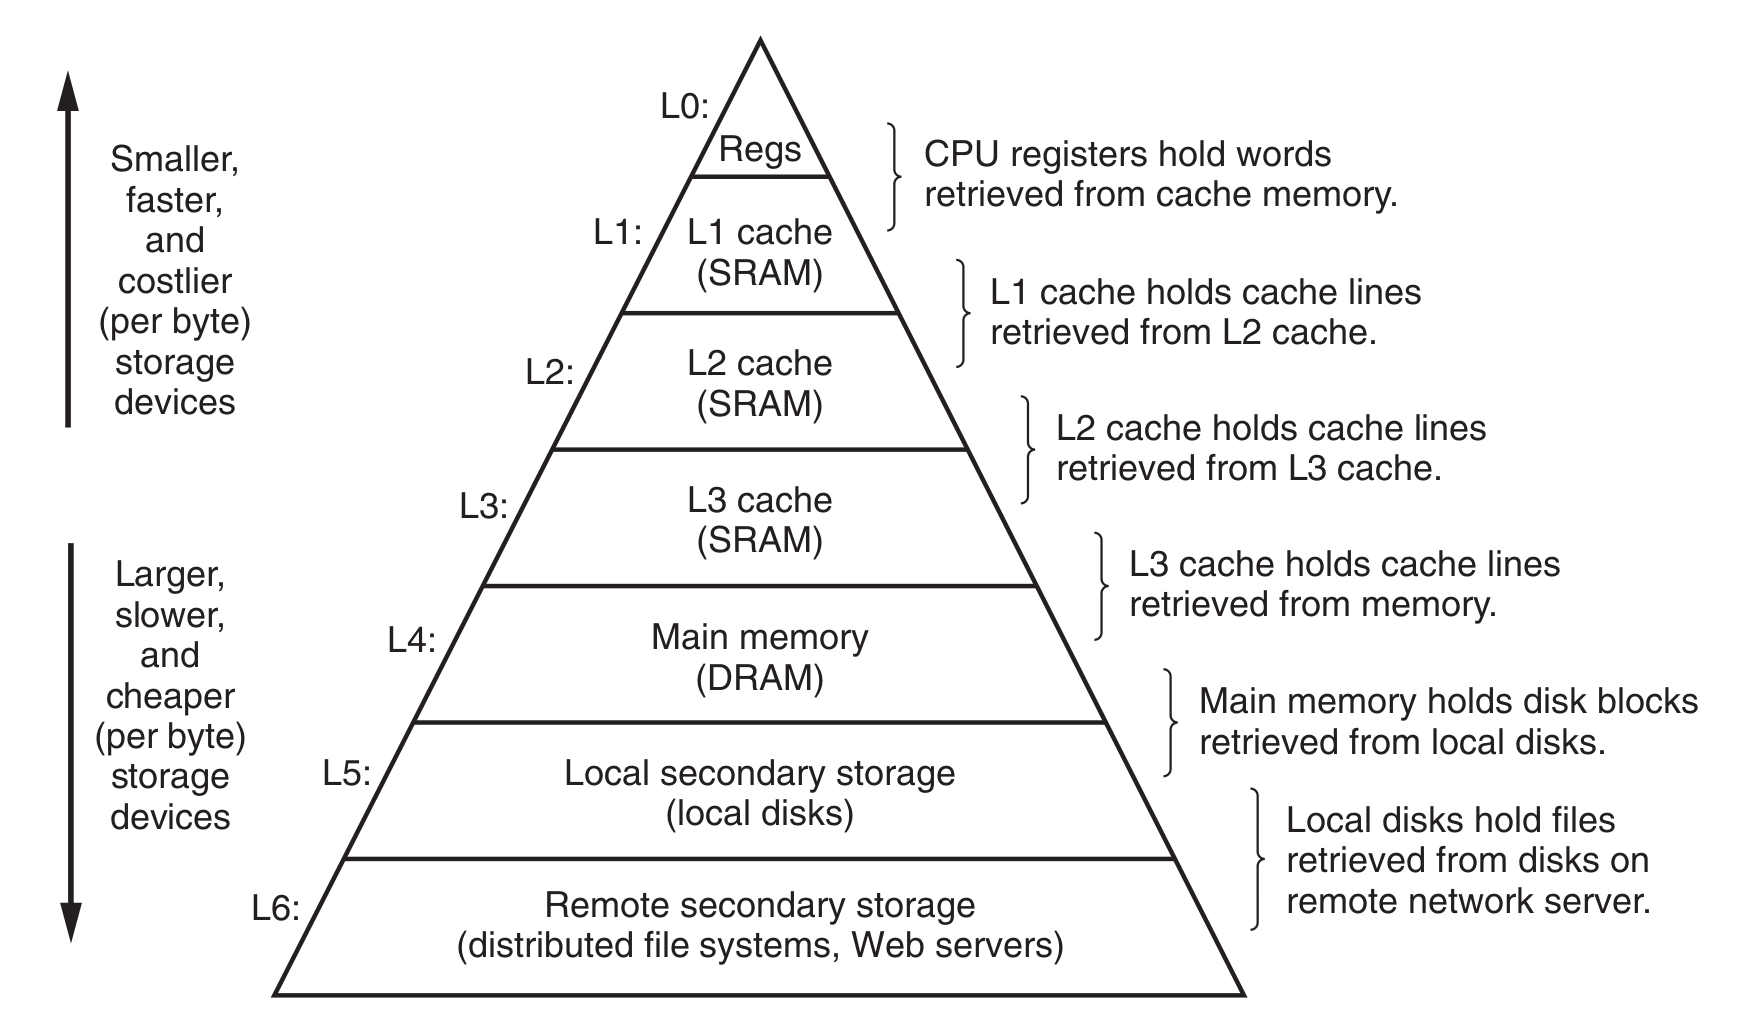
\includegraphics[width=\textwidth]{memory-hierarchy.png}
  \caption{Memory hierarchy in the operating system \cite{csapp}}
  \label{fig:memory_hierarchy}
\end{figure}

\subsection{Problems of physical memory management}

In complex systems there is a need to run multiple programs at the same time.
If~all of them were using memory directly through physical addresses, there would be problems with safety and performance.

The primary challenge with physical memory is that each process must occupy a different region of memory.
They have to use only the addresses that are inside their part of memory and shouldn't be able to modify other processes memory.
This applies to all user processes as well as the OS kernel, which memory shouldn't be even seen by user processes for safety reasons.

To address these issues, programs must be written in such a way that they can be placed at any address in memory.
There should also be hardware mechanisms designed to validate all memory accesses, ensuring that they do not violate the process's access rights.
Although there is one issue that is really hard to solve -- the memory fragmentation.
Since programs use contiguous chunks of memory, there must be a large enough contiguous memory region available for each new program loaded.
Additionally, smaller programs that consume less memory will leave small chunks of unoccupied memory after they exit.
These fragments form gaps that cannot be merged into to be used by a larger program because they are not adjacent.

There are few limitations regarding the size and number of programs running in the OS.
When the program is run, all of its memory must be in RAM occupying a contiguous region.
This means that programs cannot use more memory than is available in the system, even if they are only using a small portion of it at any given time.
Also the number of processes running concurrently is limited, because they all have some amount of memory allocated.
At some point there would be not enough free space to load a new program.

To address the last issue, some running programs may be suspended, and moved to other storage (e.g. to disk) to make room for new program.
Although such solution is inefficient, because whole memory of suspended processes must be copied to different storage (usually with higher latency).

\subsection{Virtual memory}

Virtual memory is a concept invented in 1960s by researchers working on the Atlas computer \cite{denning}.
It was designed to overcome the problems with manually maintaining the memory use of the programs.
By providing a abstraction over physical memory it enables new actions that were not possible earlier.
In this section there is an overview of main concepts used nowadays in virtual memory systems.

\subsubsection{Separate address spaces}

In systems with virtual memory all running processes have their own address space.
{\it Address space} is a set of addresses available and private to a single process.
These addresses are not real, and are not used to access main memory directly.
To distinguish the real and artificial addresses we use two different names for them: {\it virtual addresses} -- for addresses used by the process, and
{\it physical addresses} -- used to describe physical memory.
During a memory access performed by the process, the virtual address specified by the process must be translated to the physical address,
using dedicated kernel mechanism.

The use of separate address spaces makes it easier to isolate different processes.
It is not possible for a process to express the location in the address space of another process in terms of addresses known to itself.
Even if two processes use addresses that are identical because they have the same numerical value, the actual memory access is usually made
to different locations in main memory, due to address translation.

\subsubsection{Paging}

{\it Memory paging} is the technique that helps to manage memory effectively.
It divides both physical memory and virtual address space into equally sized chunks, typically 4 kilobytes large.
When we talk about physical memory, these chunks are called {\it frames}, and in virtual memory they are called {\it pages}.
Later, the virtual pages are associated with physical frames during the address translation using a page table which are both described in more details in \ref{section:address_translation}.

Each page is controlled individually and can either be in main memory or in secondary storage.
Also the location of physical frame used to store contents of memory is not relevant, because of address translation.
That means, that programs can be either partially loaded (when they operate only on few pages) or scattered across whole memory.
The ability to load only part of process memory to RAM makes it possible to run programs that use more memory than the size of RAM.

In addition to that, programs will usually start faster, because only few page has to be allocated to run the program at the beginning.
New pages, with new data or more fragments of program code, will be loaded on demand.

From safety perspective, processes has more control over attributes of allocated memory.
Each page may have different access rights specified, according to their purpose (e.g. process usually shouldn't be able to modify its instructions).
Additionally, kernel can use other page attributes to decide how it is saved or fetched form the backing storage.

\subsubsection{Memory sharing}

In system that uses virtual memory it is possible to precisely define which fragments of process memory are shared with other processes.
Such memory regions are mapped, during address translation, to the same physical pages.
Shared memory can be used to share common data, like program code or shared system libraries.
The other application is to use shared memory as a method of inter-process communication.

\section{Virtual Memory mechanisms}

There are three main mechanisms that work almost all the time when the system is running.
They provide the implementation of the concepts shown in the previous section, and work almost unnoticed by user processes.
Here we will look at the details of address translation, memory swapping, and memory fault handling.

\subsection{Memory swapping}

% DEFINED: swapped out, page daemon, backing storage, wired/pinned pages

The amount of physical memory available to the processes and kernel is limited.
Usually it is too small to store all data of all processes at the same time and sometimes even single process
may want to allocate more memory than it is physically available.
But in fact, programs don't use all of their memory at once, hence it is possible to provide different parts of memory at different times.

The illusion that all memory of the process is available in the main memory is maintained by constantly swapping unused memory pages
with the ones that are required by the process to keep running.
When a process is trying to access memory that isn't currently in RAM memory, then the page fault is triggered.
In this situation the OS kernel is responsible for finding proper page and making it available for the process.
To do this, it sometimes has to free another unused page to make a room for a new one.

To analyze the behaviour of the process in terms of using memory we define a {\it working set} to be the set of pages currently used by the process.
The working set is constantly changing over the time, but some programs have well defined stages that use different fragments of their memory.
(For example, compilers use different code and operate on different parts of the input data for different stages of compilation.)
Programmers can take advantage of this by designing programs so that the entire working set fits into main memory.
The running process will then cause as few page faults as possible, because most of the data used is already in memory.
However, if the process is poorly designed and the working set is larger than the amount of memory available to the process,
it may experience performance problems due to a high page fault rate, because used memory is constantly being swapped.
Such situation is called {\it trashing}.

%* Memory is usually not sufficient to hold all process memory \\
%  - Some other processes are using it too \\
%  - program may require large amount of memory \\
%  - but not all memory is used at once \\
%  - working set - set of pages currently used by the process (e.g. code and data used in single stage of compiler) \\
%  - when whole working set fits into memory process cause not many page faults \\
%  - When working set is too big, process will cause much more page faults. Process is trashing. \\

\subsubsection{Swapping pages}

When system is running out of space it starts to move some pages from main memory to secondary storage.
The process of moving page out of main memory is called {\it swapping out}.
To determine which pages should be swapped out kernel uses a {\it page replacement algorithm}.
The process that is walking through all pages and selecting ones to remove is typically called {\it page daemon}.

When a page is selected to be removed from memory, its contents must be stored somewhere so that the page can be recovered when it is needed again.
The place where page can be saved is called {\it backing storage} or {\it backing store}.
There are two most common backing stores: a swap partition and a file system.

Sometimes, to reduce the number of actions needed to swap out a page, kernel maintains information about modified pages.
Pages that were not modified and are already in the backing storage don't have to be copied there.
They can just be removed from main memory without losing any information about them.

\subsubsection{Page replacement algorithms}

Copying memory is expensive, especially from disks, which typically have high latency.
Therefore system is performing better when it does as little copying as possible.
There are many page replacement algorithms that are trying to achieve smallest possible number of page swaps.
All algorithms try to predict what pages won't be used in the near future, because those are the best candidates to swap out.

\begin{description}[style=nextline]
  \item[Optimal]
    The best possible strategy would be to check which page will not be used or will be used but after some time.
    Such algorithm is impossible because it requires to know future memory accesses.
    Even if that could be determined for some processes it is impossible in general.

  \item[FIFO]
    First in First out algorithm assumes, that the page that was used earlier will not be used for some time.
    In result pages are removed from the memory in the same order they were inserted.

  \item[LRU]
    Least Recently Used algorithm tries to find pages that were unused for some time.
    Kernel maintains the information about which pages were used in the past.
    Pages that were used are more likely to be used again.

  \item[Second chance]
    This algorithm implements a FIFO queue but with additional bit indicating if page was recently used.
    When some page is popped from the queue and wasn't referenced then it is freed.
    Otherwise, when its reference bit was set, it is inserted again on the page queue, with referenced bit unset.

\end{description}

%* Page replacement policies \\
%  - FIFO \\
%  - Optimal \\
%    - algorithm that requires knowledge of future access operations \\
%  - LRU \\
%    - hard to approximate in hardware \\
%    - few simplified algorithms (referenced bit, simple timer) \\
%  - Second chance page replacement alg \\
%    - FIFO on circular buffer with referenced bit \\
%    - When page is referenced, its bit is cleared and it is given a second chance \\
%    - if page is actually being used the referenced bit will be set before it will be considered again \\
%
\subsubsection{Locking pages in memory}

Sometimes there is a need to lock some pages in memory because they hold critical data or are used.
There are two categories of locked pages:

\begin{itemize}
  \item {\bf wired pages} -- such pages can't be swapped at all. Usually huge part of kernel is protected from being swapped.
    It contains critical code needed for some operations made by the kernel.
    Wired pages don't cause page fault, because they are always in the memory.

  \item {\bf pinned pages} -- temporarily wired pages of processes.
    For example, pages are sometimes pinned when a process is doing an I/O operation and its results are saved on that page.
\end{itemize}

%* Locking page in memory
%  - wired pages - in memory all the time - kernel pages
%  - pinned pages - temporarily not swappable - buffers for I/O operations done by process

\subsection{Address translation}
\label{section:address_translation}

To use virtual addresses, they must be translated into physical addresses, because main memory is addressed by physical addresses.
The translation is done by hardware unit called {\it Memory Management Unit (MMU)}, using special structures prepared by the kernel.

Every virtual address used must be mapped to a physical address, and the kernel keeps track of these mappings.
It would be impossible to describe such mappings for every single memory cell, and that is another area where memory paging helps.
Memory is divided into chunks of constant size, typically 4 kilobytes.

During address translation, the MMU splits each address into two parts: {\it virtual page number (VPN)} and {\it page offset} (figure~\ref{fig:address}).
The page number is used to find the {\it physical frame number (PFN)} in the {\it page table} -- structure managed by the kernel.
Next, the frame number and page offset are concatenated to create a physical address, which is used to reference a single memory cell.

More detailed description of address translation can be found in 7.4 of \cite{silberschatz}.

\begin{figure}
  \centering
  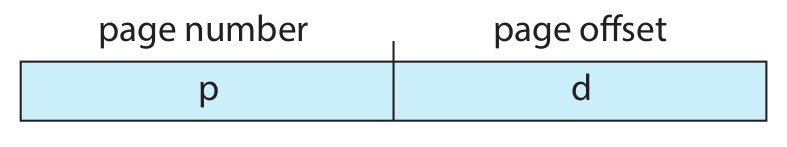
\includegraphics[width=0.5\textwidth]{address.png}
  \caption{Division of an address during address translation \cite{silberschatz}}
  \label{fig:address}
\end{figure}

\subsubsection{Page table entry details}

% DEFINED: page table entry, pte

{\it Page table entries (PTE)} are the elements of page table that describe a single mapping from virtual to physical address.
They must include all the information needed to determine physical frame location and some additional info used to check if memory access made by process is valid.
Page table entry usually contains:

\begin{itemize}
  \item {\bf Physical or virtual address}
    -- needed to identify the mapping.
    Usually only one of these addresses is stored because the second one is used to index the table.

  \item {\bf Access protection}
    -- information about operations that are allowed to perform on given memory.

  \item {\bf Valid bit}
    -- tells if the mapping is valid.
    Only valid mappings can be used by MMU to perform address translation.

  \item {\bf Address space identifier}
    -- (ASID) identifies the process which is using that page.
    Only pages with ASID matchin current process might be used to address translation.

  \item {\bf Dirty bit}
    -- determines if page was modified by the process.
    This information is used when page must be swapped out to avoid unnecessary writes to backing storage.

  \item {\bf Accessed bit}
    -- tells if any access (either read or write) was made to that page.
    This information used when searching for a page to swap out.
\end{itemize}

The set of attributes described in PTE varies between different architectures.
In Mimiker, each architecture has its own header describing the layout of the page table entries:
\href{https://github.com/cahirwpz/mimiker/blob/master/include/aarch64/pte.h}{\tt include/aarch64/pte.h},
\href{https://github.com/cahirwpz/mimiker/blob/master/include/mips/tlb.h}{\tt include/mips/tlb.h},
\href{https://github.com/cahirwpz/mimiker/blob/master/include/riscv/pte.h}{\tt include/riscv/pte.h}.

\subsubsection{Hierarchical page table}

% DEFINED: root page table, page table base register, ptbr

Conceptually, the simplest design of page table would be an array indexed with virtual addresses.
In that case, when virtual address is translated, the location of pte describing it will be easy to determine.
However, one, linear array takes too much space in memory, because every part of it must be present there, even if some regions of address space are never used.

If we assume 32 bit addresses with 4KB pages and 4 bytes PTEs, the whole 4GB address space consists of \(2^{20}\) pages.
Page table describing such address space will take 4 MB in the memory.
Because only some parts of page table are actually used, in hierarchical page tables the highest level describes which parts of page table are used.
Next levels describe smaller parts of address space, and the final lowest level consists of single page table entries.
Typically only the first level (the {\it root page table}) must be held constantly in memory, which usually takes up single page.
Other pages that hold parts of page table can either be swapped or held in memory, but even if all of them are in memory,
they took significantly less space than whole single level page table.

On the figure~\ref{fig:hierarchical_page_table} there is a scheme how physical page is found in the hierarchical page table.
The virtual address is split into few parts (the number of them depends on number of levels in page table),
and each part of it is used as an offset in next level page tables.
We start by finding a root page table, which location is usually stored in dedicated register -- {\it Page Table Base Register (PTBR)}.
In root page table, we use offset \(p_1\) to find an address of part of next level page table.
We obtain a single page of the second level page table and use offset \(p_2\) to find an address of actual physical page.
At the end, we use \(d\) as an offset in page to get final memory location.

%Hierarchical page table
%* array of PTEs indexed with virtual addresses (each virtual page have its entry)
%* describes where virtual page is in fact stored (location in main memory or non if on disk or not existing)
%
%* address space is huge -> page table would be huge
%  - calculation
%\footnote{
%  If we assume 32 bit addresses with 4KB pages and 4 bytes PTEs, the whole 4GB address space consists of \(2^20\) pages.
%  Page table describing such address space will take 4 MB in the memory.
%}.
%  - to be used by MMU the fragment containing PTE must be in memory
%  - not all fragments of pt are used (actually page tables are usually very sparse)
%  - it would be a waste of memory to allocate all pages that are creating a page table

%* page table itself is paged
%  - multi level design (number of levels depend on address space size)
%  - only top level must be in memory (other levels can be fetched on demand) (root page table
%  - calculation: for 32 bit addresses, 2 levels, first level 4KB
%
%* how pte is found
%  - parts of virtual page number (VPN) are used to index next levels of page table
%  - the last one is page offset which indicates position on a page
%  - image from silbershatz or memory systems

\begin{figure}[h]
  \centering
  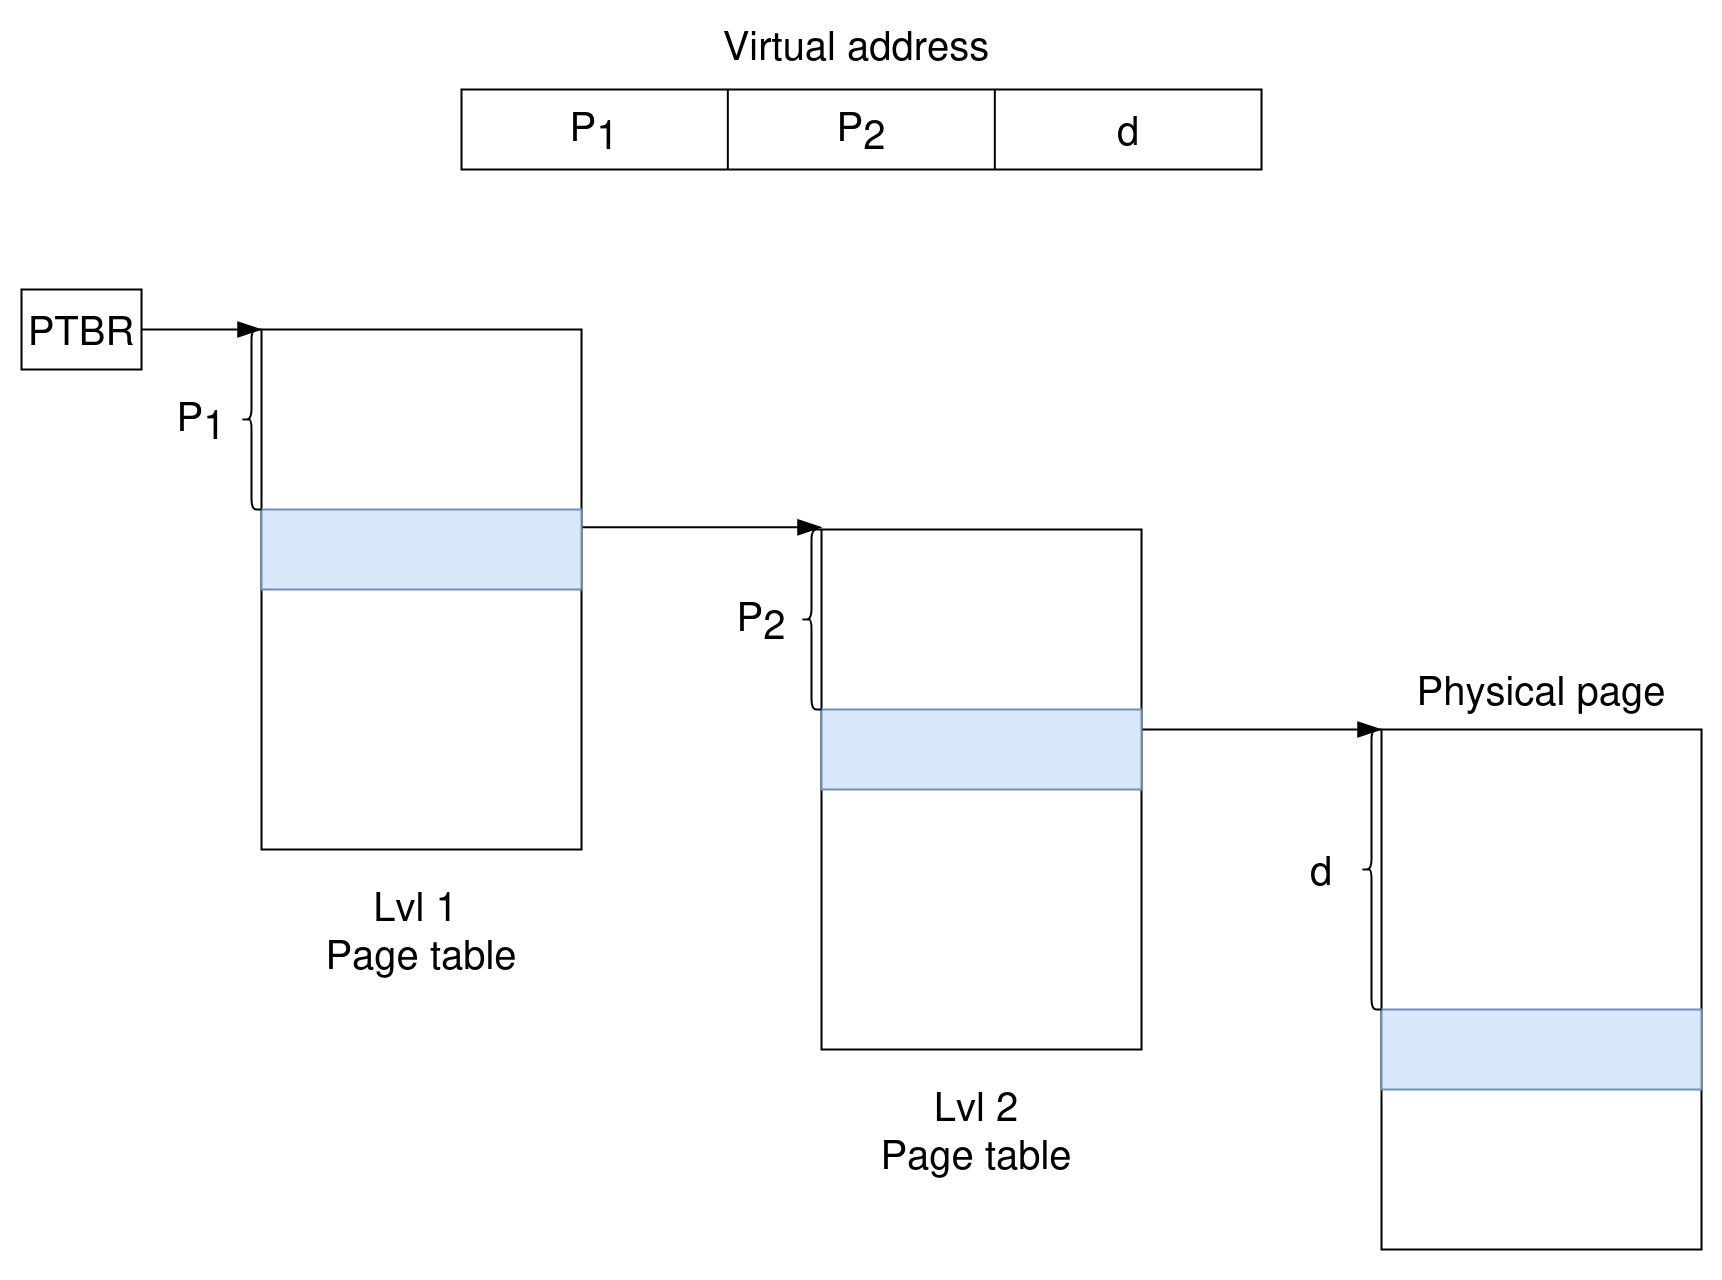
\includegraphics[width=0.7\textwidth]{hierachical-page-table.png}
  \caption{Hierarchical page table}
  \label{fig:hierarchical_page_table}
\end{figure}


\subsubsection{Inverted page table}

The inverted page tables take different approach.
Instead of defining page table for virtual address space, the table is constructed for physical memory.
The page table is in fact indexed using physical frame numbers.
The advantage over hierarchical page tables is that, the size of page table is related to the size of physical memory, and there is only one page table in the system.

Because page table is used to translate virtual addresses to physical ones, it would be hard to find page table entry knowing only virtual address.
To find proper PFN a hashing scheme is used on virtual page numbers.
Additionally, to avoid collisions, an structure called {\it hash anchor table} is used to store information about collision chains.

Inverted page tables are not common in practice, because usually it takes more memory accesses to read single PTE.

\begin{figure}[h]
  \centering
  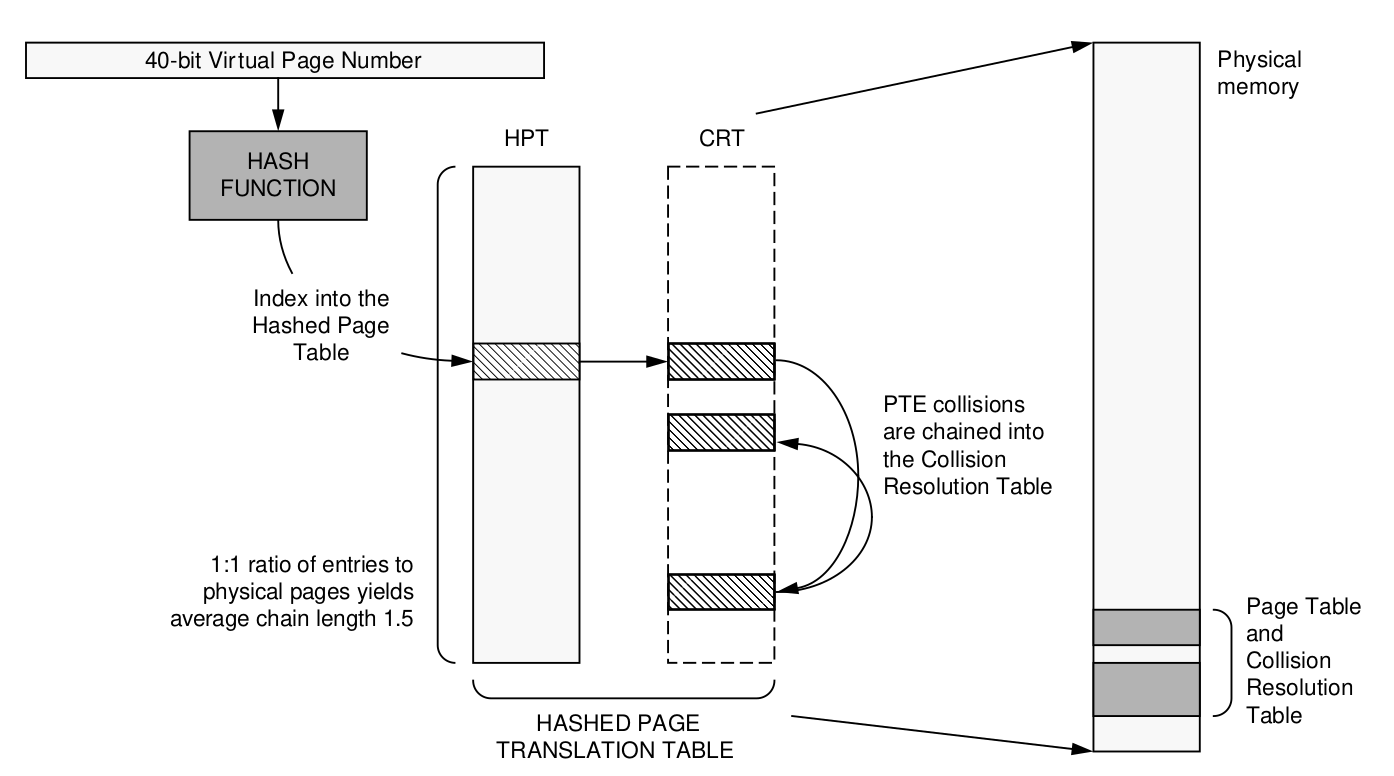
\includegraphics[width=0.9\textwidth]{memorysystems-inverted-page-table.png}
  \caption{Inverted page table \cite{memorysystems}}
  \label{fig:memorysystems:inverted_page_table}
\end{figure}

The details of page table designs, as well of real examples of their implementation can be found in \cite{memorysystems}.

\subsubsection{TLB}

The {\it translation look-aside buffer (TLB)} is a hardware designed to reduce the time it takes the MMU to read the PTEs.
It stores the most recently used page table entries because they are likely to be used again in a short time.
When making changes to the page table, kernel has to also ensure that the TLB is updated (usually by removing the modified PTEs from it).

TLB behaves like a cache for page table of current process, hence after a context switch all entries that was used by the previous process must be invalidated.
There are two ways of doing that: invalidating whole TLB after the context switch or identifying valid pages using ASID.

For more details on the design of TLB, see \cite{memorysystems}.

\subsection{Page fault}

As described in earlier sections, there are situations where memory access may fail
(either because memory is not available or because it has the wrong access permissions).
These situations must be handled by the kernel without bringing down the entire system.
When a bad memory access occurs, the {\it page fault} exception is thrown by the MMU.
The kernel must catch it, determine what caused the fault, and decide what action to take to recover from it.

We can classify page faults into 3 categories based on severity: minor and major page fault, and segmentation fault.
Minor page fault is when the page is in the main memory, but it is not referenced from page table.
In that case only page table of the process must be updated.
Major page fault happens, when page is in backing storage.
Then it has to be fetched into the main memory and proper mapping must be inserted into page table.
In the last case, the referenced page doesn't exist at all or process doesn't have a permission to perform requested memory access (e.g. write to read only page).

In fact, page faults may be triggered also by OS kernel.
Both major and minor page faults can be handled gracefully no matter in which context they happened.
The page used by kernel or user will be available after some time, because it exists.
When they happen, the page fault handler is invoked to inspect the VM~map of the process memory and determine if requested access was valid.
If that is true, the page must be made available.
By reading the VM~map of the process, it can be found where that page is stored.
There are three cases: page is actually in memory, page is in backing storage or page is not created yet.
If page does not exist it must be created or read from proper resource to be inserted into main memory.
To record information about new page or page fetched from backing storage, there must be allocated new frame in the memory and new mapping inserted into page table.

Segmentation fault cannot be handled, because it is triggered by an invalid memory access.
If it is triggered by the kernel it might cause kernel panic and bring down entire system.
When caused by the process, it isn't dangerous for the system because kernel can inform the process about it or terminate the process.
To convey the information about segmentation fault kernel sends \mintinline{c}{SIGSEGV} signal to the process.

\section{Kernel virtual memory}

In this thesis we focus on the virtual memory of user processes,
but a comment on how the kernel uses virtual memory may also be relevant.

The kernel also runs in virtual memory.
Right after it initializes all the structures needed to manage virtual memory, it switches to using virtual addresses.
This means that the kernel must also have a \mintinline{c}{pmap} structure to define the translations used by the MMU.

Even though the kernel uses virtual memory, it doesn't use all the features available to user processes.
Most of the memory pages used by the kernel are wired, and thus cannot be swapped out to make sure the kernel doesn't crash.

There are two main arguments for making kernel memory wired:
\begin{itemize}
  \item Some parts of the kernel need to be in memory at all times.
    The critical parts of the kernel may be impossible to fetch from backing storage.
    For example, if the code responsible for handling page faults is swapped out,
    it will be impossible to bring it back (because it is needed to fetch the pages from memory).
  \item There is also code that is executed very often and needs to be loaded quickly.
    If it were to be swapped out, it could cause a very long delay, which would be inconvenient for users.
\end{itemize}

Kernel memory is located at high addresses in the virtual address space.
It is always there, no matter what user process is running.
The part of pmap that describes the kernel address space is always there,
and doesn't change when process pmaps are swapped because the running process is changed.
Thanks to this, the kernel memory is always available to the kernel, no matter in which context the kernel is running.
It also allows the kernel to access the memory of the current process
(e.g. to copy some data to the buffers of the process as a result of a requested system call).

The kernel manages its memory in a different way than the processes.
It requires more sophisticated memory allocation mechanisms (e.g. slab allocators).
The details of kernel memory management are described in \cite{mckusick}, using the FreeBSD kernel as an example.


\chapter{Details of Virtual Memory subsystem}
\label{chapter:details}

In this chapter, we will look at the details of UVM, the virtual memory implementation created by Charles D. Cranor
and originally used in the NetBSD operating system \cite{cranor}.
It was designed to improve performance of virtual memory subsystem and to implement new features that were impossible to express using the old VM system.
The description of UVM here will give the details of fully working implementation in NetBSD.
The details of the implementation of UVM in Mimiker are in chapter~\ref{chapter:mimiker}.
It is essential to dive into the details of the model implementation of UVM to understand the part of it created in Mimiker.
The implementation in Mimiker is also not complete yet so this chapter will describe some features and mechanisms still not supported.
They are not yet present in Mimiker, because it would require to review and modify many other subsystems,
such as Virtual File System or interface between kernel and memory devices.

The code snippets used in this chapter are from the NetBSD sources \cite{netbsd:sources}.
To improve readability, non-essential fields have been removed from the code listings for easier analysis.

\section{Memory map of the process}

The operating system kernel must have full knowledge of the process' virtual memory map.
On the figure~\ref{img:typical-vm-map}, there is a part of typical memory map of the process.
All structures presented on that figure are used to handle all memory-related operations requested by the process.
Later in this chapter we will see all these structure in details:

\begin{samepage}
\begin{itemize}
  \item \mintinline{c}{vm_map} -- high-level description of process memory map
  \item \mintinline{c}{vm_map_entry} -- describes an individual memory segment
  \item \mintinline{c}{vm_amap} -- used to describe anonymous memory used within single segment
  \item \mintinline{c}{vm_object} -- represents a resource mapped as a memory segment (usually~a~file)
  \item \mintinline{c}{vm_aref} -- reference to an amap structure
  \item \mintinline{c}{vm_anon} -- describes a single page of anonymous memory
  \item \mintinline{c}{vm_page} -- describes a single physical page
\end{itemize}
\end{samepage}

\begin{figure}
  \centering
  \includegraphics[width=0.8\textwidth]{typical-map.png}
  \caption{Part of typical virtual memory map of the process}
  \label{img:typical-vm-map}
\end{figure}

On the top level two structures are used: \mintinline{c}{vm_map} and \mintinline{c}{vm_map_entry}.
These structures are used to properly define and manage the memory segments used by the process.

The \mintinline{c}{vm_map} stores the list of memory segments and a reference to page table structure that describes physical mappings -- \mintinline{c}{pmap}.
The \mintinline{c}{pmap} reference is used to update the mappings from virtual to physical addresses after an operation is performed on the virtual memory.
When performing an operation on the VM~map, the list of entries is usually traversed to find, insert or remove a segment.
To perform any operation on the list of segments, the VM~map lock must be held.

For the details of the VM~map structure, see the listing~\ref{code:vm_map}.

\begin{listing}
  \begin{minted}{c}
struct vm_map {
    krwlock_t lock;             /* VM map lock */
    int flags;                  /* Flags */
    struct pmap *pmap;          /* Physical map */
    int nentries;               /* Number of entries */
    struct vm_map_entry header; /* List of entries */
};
  \end{minted}
  \caption{VM~map structure}
  \label{code:vm_map}
\end{listing}

Each segment is described by a single structure -- \mintinline{c}{vm_map_entry}.
Conceptually, the VM~map entry is just a collection of pages that form a described memory segment.
Although, to make all operations on the memory more efficient a few different structures are used to maintain all the underlying pages.

The most important parts of VM~map entry structure are:

\begin{itemize}
  \item Address range -- the portion of memory that is described by this segment.
  \item Protection attributes -- the types of access allowed to the memory described by this segment.
  \item Segment flags -- the type of the segment (private or shared).
    and other attributes that define the type of memory it describes and how it must be managed (e.g. CoW segment).
  \item VM object and amap -- the structures that are used to manage the pages of the memory represented by the segment.
\end{itemize}

VM~map entries reference two types of objects that are used to store memory pages (UVM~objects and amaps)
because they are used to represent different types of memory.
Amaps describe anonymous memory, and UVM~objects represent the memory mapped files.
They create two level structure which is respected during a page lookup done during page fault.
If amap exists for a given VM~map entry, then it is the first to be searched.
Otherwise, or when page is not found in the amap, it is looked for in the UVM~object.
Amap is usually called a {\it shadowing layer} for the UVM~object.
If some page exists in both structures, its version stored in amap shadows the version from UVM~object.
This means that the version found in amap is always used to store the most recent data.
The attributes of the VM~map entry can be seen in details on listing~\ref{code:vm_map_entry}.

\begin{listing}
  \begin{minted}{c}
struct vm_map_entry {
    uint8_t flags;              /* flags */
    vaddr_t start;              /* start address */
    vaddr_t end;                /* end address */
    voff_t offset;              /* offset into object */
    vm_prot_t protection;       /* protection code */
    vm_inherit_t inheritance;   /* inheritance */
    struct uvm_object *uvm_obj; /* uvm object */
    struct vm_aref aref;        /* anonymous overlay */
};
  \end{minted}
  \caption{VM~map entry structure}
  \label{code:vm_map_entry}
\end{listing}

\section{The role of the amaps}

Anonymous memory is the memory that is released when it is no longer referenced (e.g. it has been unmapped by all processes that were using it),
because it isn't associated without any named resource like a file or device memory.
One possibility to create an anonymous memory mapping is to request one from the OS kernel using a \mintinline{c}{mmap} call.
In this case the map entry describing the requested segment contains only the reference to the amap.

The other option to create an anonymous mapping is to modify a memory in privately mapped file or other resource.
In such case, the changes made to the memory cannot be seen outside the process memory.
When the process writes to the memory page, which had to be fetched using the UVM~object, it has to be copied to the amap layer.
Because the amap layer is searched before the UVM~object, any lookups of that page will find the copy of it stored in the amap.
This ensures that all modified pages of private mappings are stored only in amaps and are freed after they are no longer in use.

\subsection{Referencing amaps from \mintinline{c}{vm_map_entry}}

Sometimes \mintinline{c}{vm_map_entries} are split into many parts
(e.g. when \mintinline{c}{mprotect} is called on a fragment of the segment to change its access protection).
After splitting, each created VM~map entry must point to a specific fragment of the original amap.
Instead of creating new amaps with content copied from the previous one, the amaps are referenced with a \mintinline{c}{vm_aref} structure.
It is a part of the \mintinline{c}{vm_map_entry} structure, and makes it possible to reference a part of the amap, specified by the offset.
If the VM~map entry is split into multiple entries, each part of it references the same amap but with different offsets.

The \mintinline{c}{vm_aref} structure is presented on listing~\ref{code:vm_aref}
and the usage of arefs during the amap split operation is pictured on the figure~\ref{img:amap_split}.

\begin{listing}[h]
  \begin{minted}{c}
struct vm_aref {
  size_t offset;
  struct vm_amap *amap;
};
  \end{minted}
  \caption{Aref structure}
  \label{code:vm_aref}
\end{listing}

\begin{figure}[h]
  \centering
  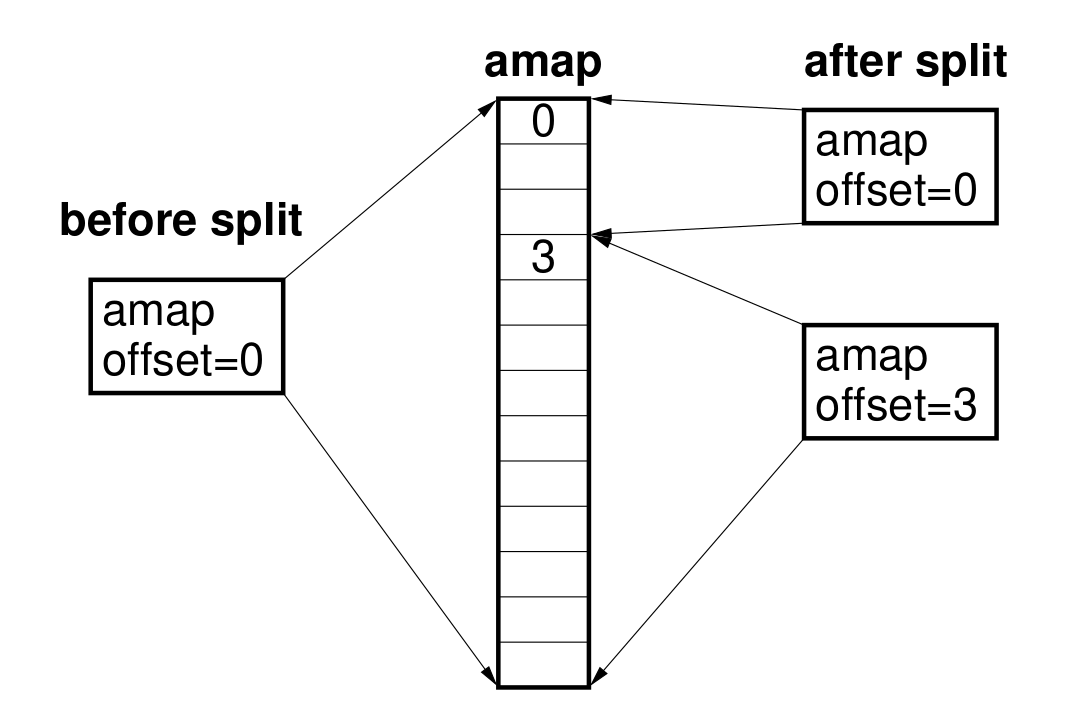
\includegraphics[width=0.5\textwidth]{amap-split.png}
  \caption{Illustration of the split of an amap \cite{cranor}}
  \label{img:amap_split}
\end{figure}

\subsection{Representing anonymous memory pages}

Individual pages of anonymous memory are described using a dedicated \mintinline{c}{vm_anon}, structure sometimes referred to as anon (listing~\ref{code:vm_anon}).
Its purpose is to make it possible to share pages between multiple amaps.
Anon structure keeps track of the number of amaps that are referencing it, in order to free the page when it is not referenced anymore.

Anons can describe resident pages as well as swapped out ones.
The pages that are already in the main memory are referenced using the \mintinline{c}{page} field.
For the pages in the backing storage the \mintinline{c}{swap_slot} number is used to retrieve them from it when they are needed again.

\begin{listing}[h]
  \begin{minted}{c}
struct vm_anon {
    krwlock_t *an_lock;      /* Lock for an_ref */
    uintptr_t an_ref;        /* Reference count [an_lock] */
    struct vm_page *an_page; /* If in RAM [an_lock] */
    int an_swslot;           /* If in swap */
};
  \end{minted}
  \caption{Anon's structure}
  \label{code:vm_anon}
\end{listing}

\subsection{Basic implementations of amaps}

Amaps store anons that represent pages that have been allocated and accessed by the process.
References to them are stored in some data structure, and single reference is saved in an {\it amap slot}\footnotemark.
\footnotetext{
  Amap slots are entirely different concept than the backing storage slots.
  Thy describe the location of anons and are used to represent location of the anon in virtual memory address space.
  In contrast, backing storage is used to store raw content of memory pages that were swapped out.
  The swap slot number, which is recorded in the anon structure, is the location of memory of given page in the backing storage.
}
Slots may be active, when they have valid reference to an anon, or inactive, when they don't hold any anon.
Typically, amap slots are inactive if the portion of memory that would have been described by the anon referenced by the given slot
is described by the UVM~object or hasn't been accessed by the process yet.
We access individual slots using the index ({\it slot number}),
which is calculated from the virtual address of the memory that is within the range represented by the given amap.

Operation on amaps are performed using amap API, which makes it possible to provide different implementations of amaps.
When adjusting the OS kernel to run on some constrained machine, the most efficient implementation may be chosen.
Later we will see three different implementations of amaps.

The most important operations defined in the amap API:

\begin{itemize}
  \item \mintinline{c}{amap_alloc} and \mintinline{c}{amap_free} -- allocate new amap and free one
  \item \mintinline{c}{amap_ref} and \mintinline{c}{amap_unref} -- increase and decrease reference count of the amap
  \item \mintinline{c}{amap_extend} -- increase the size of amap
  \item \mintinline{c}{amap_add} and \mintinline{c}{amap_unadd} -- add and remove anons from amap
  \item \mintinline{c}{amap_lookup} -- search for anon
  \item \mintinline{c}{amap_copy} -- make a shallow copy of the amap (anons are not copied, but referenced from both original and new amaps)
  \item \mintinline{c}{amap_cow_now} -- make a deep copy the amap (every anon referenced from the amap is also copied)
\end{itemize}

The two basic implementations, array-based and list-based, are described below.
They are also presented on figures \ref{img:array-amap} and \ref{img:list-amap}.

\subsubsection{List based amaps}

This implementation uses a list to store references to \mintinline{c}{vm_anon} structures.
It will use exactly as many slots as needed, so it could be used if the system is running on a memory-constrained device.
Mass operations on the anons stored in the amap are fast
(looping through the list is efficient, because all visited list elements represent the anons that are actually being used).
On the other hand, operations on individual anons can be slower (finding a specific anon in the list requires iterating over the whole list).

\subsubsection{Array based amaps}

This implementation stores pointers to \mintinline{c}{vm_anon} structures in the array indexed by the slot number.
It also keeps track of active slots (the slots that hold already used anons).
Here, operations on single anons are fast (knowing the offset of the anon allows to get it instantly from the array).
Iterating over all active anons is now slower, because all slots have to be checked.

\begin{figure}
  \centering
  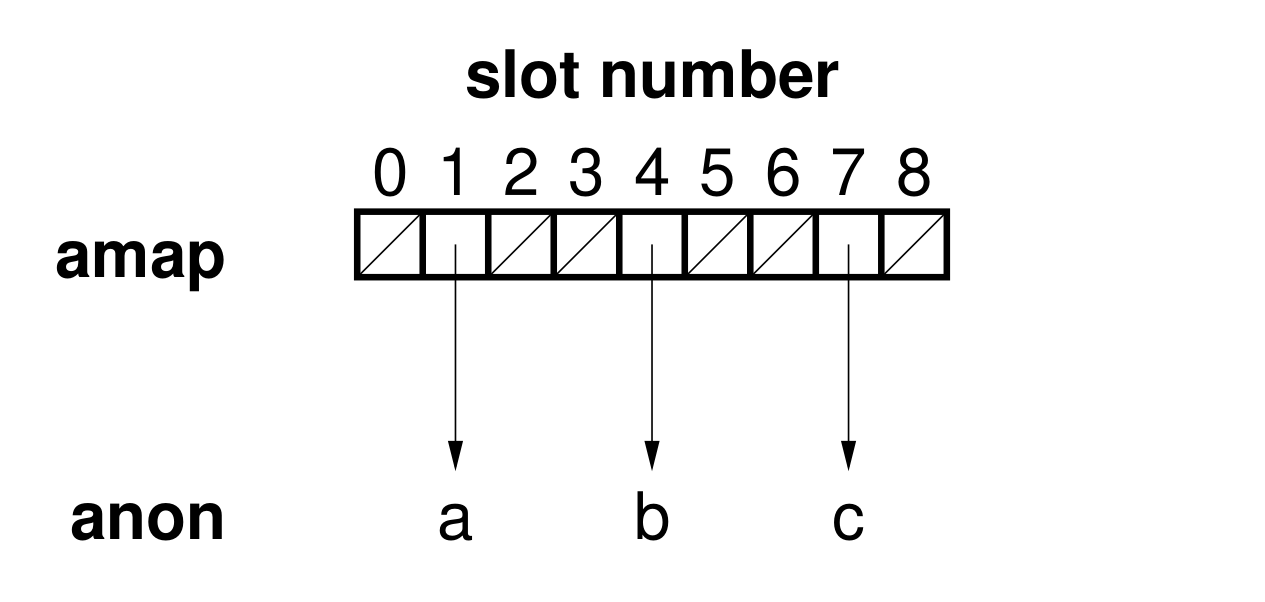
\includegraphics[width=0.5\textwidth]{array-amap.png}
  \caption{Amap implementation with an array of anons \cite{cranor}}
  \label{img:array-amap}
\end{figure}

\begin{figure}
  \centering
  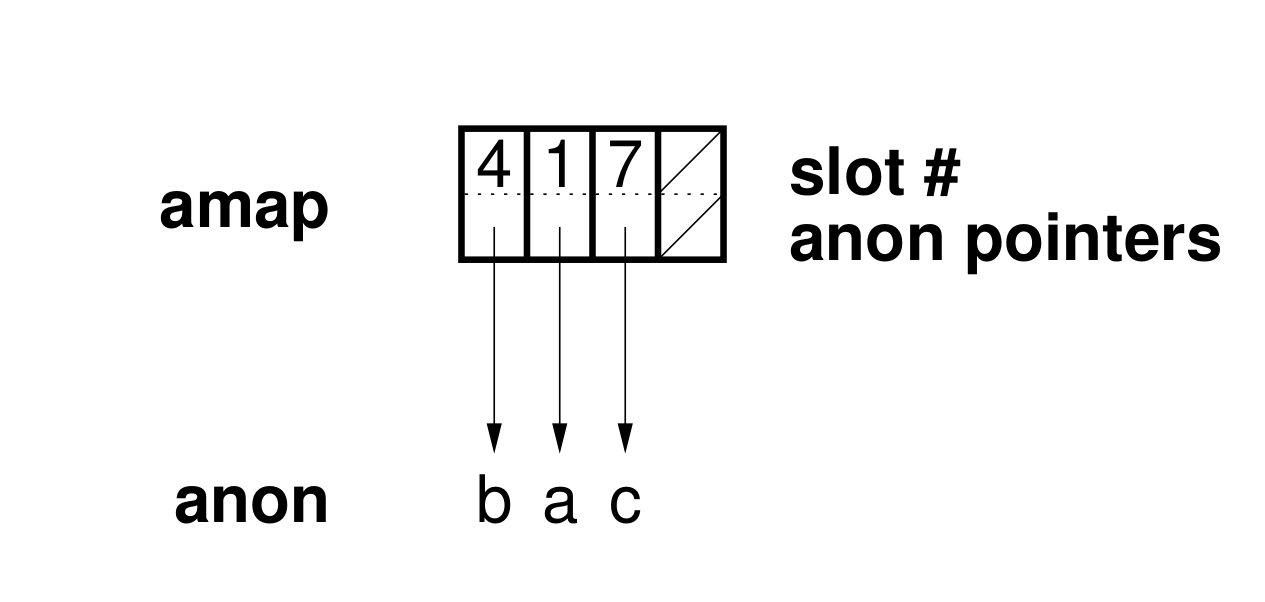
\includegraphics[width=0.5\textwidth]{linked-list-amap.png}
  \caption{Amap implementation with a list of anons \cite{cranor}}
  \label{img:list-amap}
\end{figure}

\subsection{Implementation of amaps used in UVM}

Both of the above implementations of amaps are good at one type of operation, but slow at others.
UVM uses a different approach.
It combines both implementations to create a one that is efficient in all types of operations.
The disadvantage is that it uses more memory (it needs 3 arrays instead of 1).

\mintinline{c}{vm_anon} structures are stored in the array indexed by slots (\mintinline{c}{am_anon}).
Slot numbers of active anons are stored in the list (\mintinline{c}{am_slots}).
To synchronize these structures the third one (\mintinline{c}{am_bckptr}) is used.
For each active slot, it stores its position on the list.
It is used to update the list of active anons when an anon is deleted.
The relations between all these three arrays are presented on figure~\ref{img:uvm_amap_impl}
and the C structure that describes the amap is on the listing~\ref{code:vm_amap}.

\begin{figure}
  \centering
  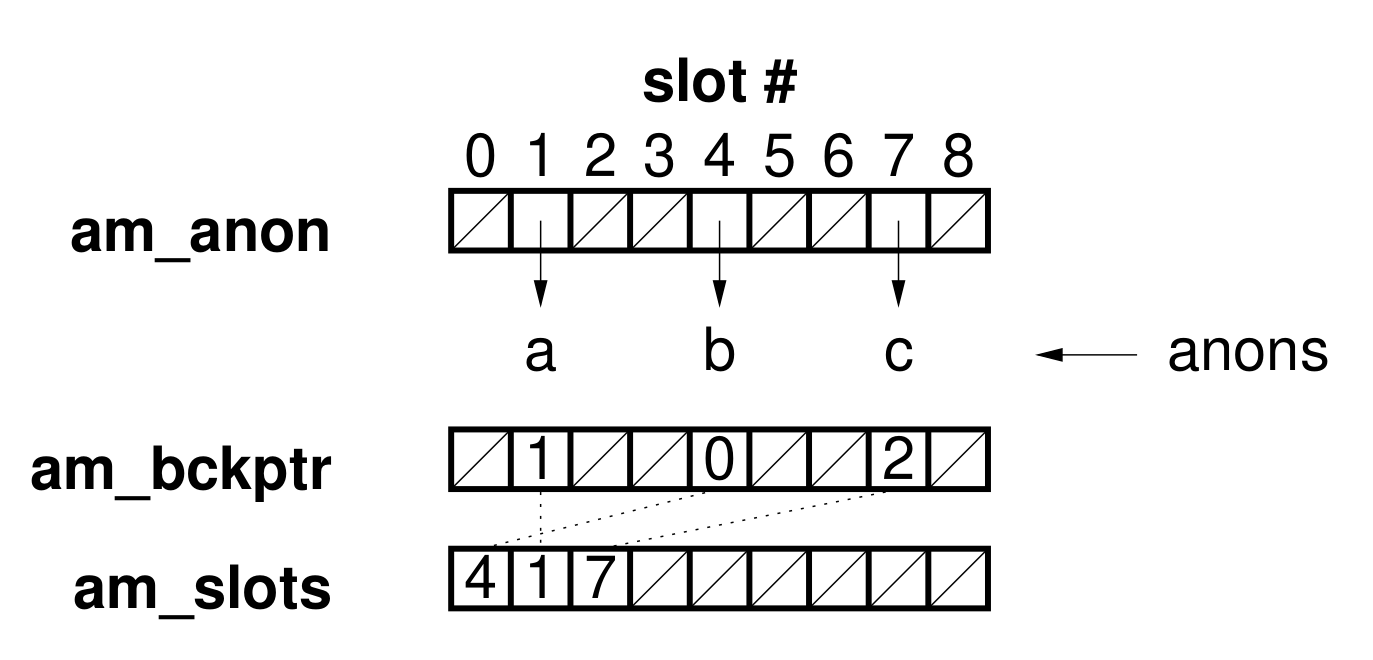
\includegraphics[width=0.5\textwidth]{uvm-amap.png}
  \caption{Amap implementation used in UVM \cite{cranor}}
  \label{img:uvm_amap_impl}
\end{figure}

\begin{listing}
  \begin{minted}{c}
struct vm_amap {
    krwlock_t *am_lock;       /* lock [locks all vm_amap fields] */
    int am_ref;               /* reference count */
    int am_flags;             /* flags */
    int am_maxslot;           /* max # of slots allocated */
    int am_nslot;             /* # of slots currently in map  */
    int am_nused;             /* # of slots currently in use */
    int *am_slots;            /* contiguous array of active slots */
    int *am_bckptr;           /* back pointer array to am_slots */
    struct vm_anon **am_anon; /* array of anonymous pages */
};
  \end{minted}
  \caption{Amap structure}
  \label{code:vm_amap}
\end{listing}

\begin{samepage}
\section{The role of the UVM~object}

Memory segments in the VM~map of the process may also represent the memory of files and devices.
To properly manage them and keep in sync with the actual memory of the resources there is a need for another structure.
  UVM~object structure, presented on listing~\ref{code:uvm_object}, holds three types of information:

\begin{itemize}
  \item A structure to keep track of the pages that are resident, along with a total number of them (\mintinline{c}{uo_npages} and \mintinline{c}{uo_pages}).
  \item The number of references from VM~map entries to that object (\mintinline{c}{uo_refs}).
  \item The reference to pager operations for given type of UVM~object (\mintinline{c}{pgops}).
\end{itemize}

\end{samepage}

\begin{listing}[h]
  \begin{minted}{c}
struct uvm_object {
    struct krwlock *vmobjlock;  /* lock on object */
    int uo_npages;              /* # of pages in uo_pages */
    unsigned uo_refs;           /* reference count */
    struct radix_tree uo_pages; /* tree of pages */
    const struct uvm_pagerops *pgops; /* pager ops */
};
  \end{minted}
  \caption{UVM~object structure}
  \label{code:uvm_object}
\end{listing}

UVM~objects represent the memory of some resource, hence they need to reference that resource in some way.
Instead of using dedicated structure field to record that the author of UVM decided to express it differently.
Every resource that can be mapped into process's memory has an UVM~object structure embedded into its structure.
As a result, knowing what type of resource is connected with given UVM~object we can calculate the address of that resource, based on the address of UVM object.
Actually, to make it even more direct, the UVM~object is saved at the beginning of the structure (as its first field).
On listing~\ref{code:vnode} there are a few initial lines of \mintinline{c}{struct vnode} definition, that shows the inclusion of UVM~object into vnode structure.

\begin{listing}[h]
  \begin{minted}{c}
struct vnode {
    struct uvm_object v_uobj;
    voff_t      v_size;
    /* Other fields ... */
};
  \end{minted}
  \caption{Part of the \mintinline{c}{vnode} structure}
  \label{code:vnode}
\end{listing}

\subsection{Pager interface}

Pagers define how operations are made on different types of UVM~objects.
The operations possible to perform are described by the {\it pager interface}, but each pager type provides its own implementation of them.
There is exactly one pager defined for each type of UVM~objects, and they are initialized during a system startup.
Every UVM~object references one structure which has the references for pager operations suitable for object of given type.
Because all operations on UVM~objects are conducted via the pager interface, there is no need to explicitly save the type of UVM object inside its structure.
By referencing a set of dedicated pager operations, the proper implementation of requested operation is executed.

Operations defined in the pager interface:
\begin{itemize}
  \item \mintinline{c}{pgo_init}
    -- Initialize the pager private data structures (e.g. the linked list of all allocated device-backed objects).
       Used only once for each pager during boot.

  \item Attach operation used during the creation of UVM~object.
    -- Each pager type defines its own attach function which performs all actions needed to obtain UVM~object of given type.
       (E.g. \mintinline{c}{uao_create} -- for anonymous UVM~objects,
             \mintinline{c}{udv_attach} -- for device-backed UVM~objects, and
             \mintinline{c}{uvn_attach} -- for vnode UVM~objects.)

  \item \mintinline{c}{pgo_reference}
    -- Increase reference count of the object.

  \item \mintinline{c}{pgo_detach}
    -- Decrease reference count of the object.

  \item \mintinline{c}{pgo_get}
    -- Get page from the object or read it from the backing storage.
       Typically called during page fault.

  \item \mintinline{c}{pgo_fault}
    -- Custom fault processing routine used when \mintinline{c}{pgo_get} isn't enough.

  \item \mintinline{c}{pgo_put}
    -- Write dirty page to the backing storage.
       Usually performed by the page daemon.

\end{itemize}

\subsection{Pager types}

UVM~object are distinguished only by looking at their pager operations.
There are three types of objects defined in UVM:

\begin{description}[style=nextline]
  \item[Vnode pager]
    Used when VM object is representing a file mapped into the process memory.

    It is the most used pager because most of memory is a memory of files (e.g. program code, and shared libraries)
    and provides an efficient way to make files I/O operations.

  \item[Device pager]
    Memory pages reflect the memory of given device.
    It is usually used to make operations on devices easier (e.g. write directly to the frame buffer memory).

  \item[Aobj pager]
    Anonymous memory object pager.
    Although anonymous memory of the process is handled entirely using amaps, there are some situations when it isn't enough.
    The memory pages that are fetched from aobj into the memory map of process are treated as any non-anonymous memory pages.
    The difference is in the resource they come from.
    Anonymous objects are used in resources that are temporary and will not be saved after they are no longer used in the system.
    Good example here is a tmpfs.
    The file system which is cleared when the OS is shut down, because it lives only in the RAM memory.

\end{description}

\section{Using UVM to serve page fault}
\label{uvm:page_fault}

When a program wants to use some memory (using a virtual address), the MMU checks its page table to figure out the actual location in the physical memory.
If the page table has the right information for the given virtual address, and the access permissions are correct,
the program can access the memory without any additional action from the kernel.
However, if the page table doesn't have the needed information or the program is trying to access memory it shouldn't (for example writing to read only memory),
a page fault happens, and the kernel has to step in to fix things.

When handling a page fault, kernel uses the VM~map to check whether the memory access was valid or if the process needs to be notified about the fault.
It uses the structures mentioned above to locate the page if it already exists, or if it needs to be created or fetched from backing storage.
The description of page faults in this section doesn't take into account the copy-on-write mechanism.
This is discussed in the next section.

The lookup is started at the \mintinline{c}{vm_map} level by traversing the list of \mintinline{c}{vm_map_entries}.
After finding the map entry containing the faulting page,
it is possible to check whether the process was allowed to make the desired memory access.
If the protection flags are incompatible with the type of access made by the process,
the procedure is aborted and the process receives \mintinline{c}{SIGSEGV} with additional code \mintinline{c}{SEGV_ACCERR}.
If the map entry is not found in the memory map of the process,
the \mintinline{c}{SIGSEGV} is sent with \mintinline{c}{SEGV_MAPPERR}.

Now the found VM~map entry is used to fetch the desired page.
Since there are two levels at which the page can be found,
we must search these levels in the correct order: first in the amap, then in the UVM~object.

In amap, pages of anonymous memory are represented by anons.
If there is an anon at the offset specified by the faulting page address, then the actual page is referenced by it.
If anon has a pointer to the \mintinline{c}{vm_page}, then that is the page we are looking for.
Otherwise, anon has a swap slot number assigned, which tells where the page content is stored in the swap space.
The new physical page must be allocated and filled with data read from the swap slot.

If there is no anon at the specified offset, we must look for the page in the UVM~object.
Here, there also two possibilities, the page might be present in the UVM~object or must be fetched from the backing storage.
In the latter case, the pager interface associated with the UVM~object is used to fetch the desired page.

In both cases, when correct page is allocated and filled with proper data, kernel must update the page table mappings described in \mintinline{c}{pmap}.
This action is done using \mintinline{c}{pmap_enter} function with the found page as an argument.
The attributes of created mapping depends on the VM~map entry type (whether it is shared or private) and access privileges described also there.

\section{Copy-on-Write mechanism in VM}

Copy-on-write, as described at the beginning, is used to reduce number of page copies and share private memory of processes for as long as possible.
It takes it action when private memory segments are copied (during {\tt fork}) and accessed (when they trigger a page fault).
Before the first write, pages of the memory mapped file can be shared with others.
To achieve this, the segment with private mapping must be marked as CoW, and then it will behave like any other CoW mapping.

There are two moments in the life of the operating system where copy-on-write takes action: the \mintinline{c}{fork} syscall and the page fault routine.
These are the moments when the kernel decides what memory is accessible to the process and what memory protection is used for the memory mappings.
CoW mechanism implements new rules that must be followed when performing these actions.

\subsection{Forking with CoW in mind}

When copy-on-write is implemented, then the fork operation is different than usual.
There is much less copying to do because the private memory segments, which were previously copied,
can be shared for some time, and copied only when it is truly needed.
During the creation of the new process, only the \mintinline{c}{vm_map} and \mintinline{c}{vm_map_entries} are copied to build the VM~map of the new process.
After fork the same amaps and UVM~objects are referenced from structures in both child and parent processes.
Thanks to that, fork is usually faster, because we avoid a lot of copying.

To distinguish shared memory from private memory, which is shared only until the first write,
the kernel must record some additional information about memory segments.
There are two flags that are set on the private VM~map entry during a fork:

\begin{itemize}
  \item \mintinline{c}{COPY_ON_WRITE} -- indicates that the segment is CoW.
    This means that before writing to the memory, it must be ensured that it has been copied
    and that the write operation will not be seen by other processes (especially parent or child).
    This flag remains set until the VM~map entry is destroyed.
  \item \mintinline{c}{NEEDS_COPY} -- indicates that the amap used by this item must be copied
    before any page is inserted into it (or created if it doesn't already exist).
    This flag is cleared immediately after the amap is copied.
\end{itemize}

Another thing that must be done during the fork is to change the access protection for the parent process to some pages.
From now, some of the memory regions must be copied before the first write to them.
To enforce this, the write access is removed from the page table entries of the pages described by these segments.
Thanks to that, when the parent process tries to write to those memory segments, it triggers a page fault
(because MMU has information that writing there isn't allowed).
During a page fault, the action must be taken to copy this memory and allow the process to write to it again.

However, copy-on-write can't be used on all private memory segments.
Process may mark its memory segments to be resident in main memory all the time (such memory is then called wired).
This is done to avoid additional overhead caused by page faults when some page must be fetched from backing storage.
When such memory segment is discovered during a {\tt fork} operation, its memory must be immediately copied to be accessible by the child process
without causing any page fault.
In that case the \mintinline{c}{amap_cow_now} function is used to ensure all pages referenced by an amap are copied and ready to use.

The segments that represent wired memory cannot cause any page fault
(neither page fault caused by wrong access protection nor by the lack of memory pages in the RAM).
Because of that, we would not be able to limit the access protection for them.
Such memory segments must be copied during a fork, using a \mintinline{c}{amap_cow_now} function.

After the VM~map was cloned, both parent and child processes can start executing.
The original process is executing using its original pmap during address translation.
The child process obtains its own, empty page table, which is filled in while the process executing.
Due to paging, new entries are added to the page table during page faults caused by memory accesses to child memory.

\subsection{Page fault handling in CoW scenario}

In this section we will see in details how page fault is handled when it occurs on the memory marked as CoW.
Due to the design of the memory map, the faulting page can be found at two different levels.
Moreover, the operations needed to ensure that page is correctly found, copied and inserted into process page table are different
for different access types that caused a page fault.
There are actually 3 different types of access operations: read, execute and write, but page faults caused by them are divided only into two categories.
Read and execute accesses both generate {\it read page fault} because they both read memory (either data or instructions) and,
more importantly, they don't modify the memory being accessed.
{\it Write page fault} is another type of fault, generated by write accesses, because it modifies memory contents.

\subsubsection{Read page fault}

Read fault is easier to handle, because there are less actions to perform.
When a page is found, either in amap or UVM~object, it can be inserted into the process page table without copying it.
However, the access protection assigned to that page must be carefully tweaked, if the original access protection allows for write operations on it.
If the page is still used by different processes, then it can't be written by any of the processes that share it,
hence we need to remove write access right from it to trigger a page fault on a first write operation on it.

We can determine if the page is shared between processes, by checking the reference count of the structure that is holding that page:
\begin{itemize}
  \item If it is held by anon, we need to check if anon or amap are shared,
  \item If it is held by UVM~object, then we need to check if the UVM object is shared.
\end{itemize}

\subsubsection{Write page fault}

As mentioned multiple times earlier, the OS kernel must copy the page shared because of copy-on-write mechanism before it is modified by the process.
Therefore, when we encounter a page fault due to write access on the memory marked as copy-on-write, we need to ensure that the process has its private copy of it.

At the beginning, we have to ensure that the amap is private for the current process.
If it's still shared between multiple processes, and the \mintinline{c}{NEEDS_COPY} flag is set in the amap flags, it must be copied.
As a result, all the anons referenced by the amap will have their reference counter bumped to reflect that they are now referenced by one more amap
(by the original one, and by the new copy of the amap).
There is also the possibility that the amap hasn't been created yet.
In such case it must be allocated.

Now there are three different cases depending on where the page was found:

\begin{description}[style=nextline]
  \item[Page in the UVM~object]
    The UVM~object is shared between multiple processes.
    Because we are in CoW scenario the page that is found there must be copied to create a copy of it private for the current process.
    The copy of the page is saved in the amap that is referenced from the same VM~map entry as the current VM object.
    Recall that the amap was previously copied or created so it must be private for the current process.

  \item[Page in the anon shared between multiple amaps]
    The page is shared between many processes, because some of them hasn't still made a write access to that page, because they haven't created a copy of it yet.
    All other processes that has access to current page shouldn't see the modified memory, so the page must be copied.
    We create a new anon holding the page copy and insert it into the amap instead of the old one.
    The reference count of the old anon is decreased and if it drops to one.

  \item[Page in the anon private for current amaps]
    This situation is possible, when the process that encountered a page fault is the last one holding found page.
    It means, that all other processes have their own copy of it created earlier so the reference count of the current anon is equal to one.
    In such case, the page doesn't need to be copied, and can be inserted into page table with full access rights.

\end{description}


%\subsubsection{CoW on page found in the UVM~object}
%
%In this case, the UVM~object is shared by multiple processes and access to that page triggered a page fault.
%It can be caused by either read or write operation.
%In each of those cases there are different steps to perform:
%
%\begin{enumerate}
%  \item {\bf Read fault}\\
%    The page is inserted into the page table with removed write access.
%    This is done to make it possible to copy this page before the first write occurs.
%    The write operation on that page will trigger another page fault (described in the next step)
%
%  \item {\bf Write fault}\\
%    The page is copied and added to the amap.
%    In this case, the amap must be private for the process that is using it.
%    The process of ensuring that is described in next section.
%    It can be inserted with full access rights, because from now it is a private copy of that page for a process.
%\end{enumerate}
%
%\subsubsection{CoW on page found in the amap}
%
%If a page fault is triggered by a read operation, it is handled the same way as described in the previous section.
%The protection is limited and the page is inserted into the pmap.
%Otherwise, when the process tries to write to that page, we can distinguish several cases:
%
%\begin{enumerate}
%  \item {\bf Amap is shared between multiple processes}\\
%    Both processes are referencing the same amap.
%    Such situation happens right after the fork has succeeded.
%
%    Initially, we check if the flag \mintinline{c}{NEEDS_COPY} is set.
%    If multiple entries reference the amap, it should be copied.
%    Consequently, all the anons referenced by the amap will have their reference counter bumped
%    (to reflect that they are now referenced by one more amap).
%    Next, the anon that is storing the faulting page is copied and inserted into the new amap.
%
%  \item {\bf Anon is shared between multiple amaps}\\
%    The anon is still shared between multiple amaps, when it wasn't written by any of the processes, but some other
%    anon was copied, and in result the amap was copied.
%    In this case, each process has its own copy of the amap, so only the anon needs to be copied.
%    Then, the new anon is inserted into the amap.
%
%  \item {\bf Everything is copied}\\
%    Both amap and anon are copied, when the other process has previously encountered a page fault accessing given page.
%    It has been copied by the other process, so the current one has nothing to do.
%    The found page is inserted into pmap without any copying.
%\end{enumerate}

\section{Interaction with page table}

The VM subsystem manages the virtual memory of the processes,
so it must ensure that the virtual address space is correctly mapped to physical memory.
After each change to the process virtual memory map, it must update the page table used by the modified process.
This is not always done immediately after the virtual memory map is changed.
Sometimes, such as when a new memory mapping is created, the page table is modified during a page fault caused on that region.
The VM subsystem is a machine-independent module, so it must interact with the pmap
-- the machine-dependent part responsible for updating the page table.

Other kernel modules interact with pmap through an interface that defines a set of functions used to create, remove and modify page table entries.
Below are the functions used by the VM subsystem to manage physical mappings.
The addresses passed to these functions as parameters are used to describe pages, therefore they must be page aligned.

\begin{description}[style=nextline]
  \item[{\tt int pmap\_enter(pmap\_t pmap, vaddr\_t va, paddr\_t pa, vm\_prot\_t prot, \\ u\_int flags)}]
    Create a new mapping in the given {\tt pmap}.
    {\tt va} and {\tt pg} specify the virtual address and physical page that are part of the mapping.
    {\tt prot} and {\tt flags} describe additional attributes of the created mapping.

  \item[{\tt void pmap\_remove(pmap\_t pmap, vaddr\_t start, vaddr\_t end)}]
    Remove the existing mapping from the pmap.
    The removed region is described by virtual addresses {\tt start} and {\tt end}.

  \item[{\tt void pmap\_protect(pmap\_t pmap, vaddr\_t start, vaddr\_t end, vm\_prot\_t prot)}]
    Change the memory protection bits of the memory between the virtual addresses {\tt start} and {\tt end}.

  \item[{\tt void pmap\_copy\_page(paddr\_t src, paddr\_t dst)}]
    Copy the contents of one physical page ({\tt src}) to the other ({\tt dst}).

  \item[{\tt pmap\_t pmap\_create(void);}]
    Create a new page table.

  \item[{\tt int pmap\_fault\_handler(ctx\_t *ctx, vaddr\_t vaddr, vm\_prot\_t access);}]
    This is not part of the interface, but the function used to handle a page fault.
    The handled page fault has occurred on virtual address {\tt vaddr} by the access type specified with {\tt access}.
    This function sometimes triggers the VM function used to handle the page fault at VM level.
\end{description}

\section{The old BSD~VM system in NetBSD}

Prior to the creation of UVM, NetBSD used a different VM subsystem.
The reason for understanding the concepts of the old implementation is that the VM subsystem used before in Mimiker was also based on it.
Throughout this chapter, the old VM subsystem will be referred to as BSD~VM, while the current one will be referred to as UVM.

The BSD~VM implementation focuses on utilizing VM objects, structures in some way similar to UVM~objects, to serve all operations on virtual memory.
This section will show the high level overview of the design of the BSD~VM.

\subsection{Overview of the design}

The BSD~VM system also uses the VM~map structure to describe the process virtual memory map.
Single segments of process memory are described with VM~map entries.
The structure of a VM~map entry is very similar to the structure used in UVM, although it has only
the reference to single VM object (because there are no other structures to describe the memory).
To describe physical pages, UVM and BSD~VM use an almost identical structure.

The big differences between the two discussed virtual memory implementations are seen during the fork and page fault routines.
Hence the main components of the VM implementation, the structures that hold VM pages, are very different,
the process of searching for pages, copying and replacing them must also be different.

\subsection{VM objects structure}

The VM objects are used to represent the memory of a single resource available in the system (e.g. a file) or the anonymous memory.
They maintain the information about all memory pages that hold the data fetched from the represented source.
They are also needed to properly handle all operations when swapping a page out or fetching it from a backing storage.
The location of the backing storage is determined based on the VM object type.

Even if the names of VM object and UVM~object are similar, they work differently.
Hence, the VM object is the only structure used to store VM pages, it is larger than UVM~object.
The UVM~object is embedded in the structure of the resource, while the VM object has a special handle to it.
The VM object structure definition (still used in the FreeBSD system) is almost 100 lines long,
while the UVM definition (presented earlier on listing~\ref{code:uvm_object}) has less than 10 lines.

Hence VM objects are used to represent all memory of processes in the system, there are three types of them:

\begin{description}[style=nextline]
  \item[Named VM objects]
    Used to represent named resources available in the operating system.
    These resources are used to fetch the memory pages and to save them when they are modified.
    The most common resources that are mapped into memory are files, but there are others,
    for example memory of hardware devices like frame buffers.
  \item[Anonymous VM objects]
    Used to represent the memory that is filled with zeros before being used.
    The memory isn't associated with any resources in the system.
    After the objects is no longer used, the memory is destroyed without saving it anywhere.
  \item[Shadow VM objects]
    These objects main purpose is to provide a shadowing layer for other VM object.
    They reference the other VM object and hold the copy of its pages that were modified by the process but the changes shouldn't be
    reflected in the original resource.
    This type of VM objects are essential to implement private memory mappings and copy-on-write.
\end{description}

The important part of the VM object, that defines its type, is a {\it pager interface} used by the object.
Pager interface defines operations that operate on the backing storage associated with given VM object:

\begin{itemize}
  \item Read a page from the backing storage.
  \item Write the page to the backing storage.
  \item Check if page is present in the backing storage.
\end{itemize}

Hence there are a few backing storages types, there are also a few types of pager interfaces:

\begin{itemize}
  \item Vnode pager -- used to provide memory mapped files using the vnode that represent the file.
  \item Device pager -- handles operations on device memory represented by the VM object.
  \item Swap pager -- used for anonymous memory. It reads and writes pages from swap space.
\end{itemize}

The information stored in the VM object structure:
\begin{itemize}
  \item The collection of memory pages resident in main memory.
    There are usually two structures for holding these pages:
    a radix tree (for fast random access) and list (for fast iteration over all pages).
  \item Many different metrics:
    \begin{itemize}
      \item Number of resident pages
      \item Total size of represented resource
      \item Number of references to the object (from different VM~map entries).
    \end{itemize}
  \item The pager data:
    \begin{itemize}
      \item The type of pager.
      \item A handle to resource (typically a vnode structure)
      \item Pager private data.
    \end{itemize}
  \item Reference to the other VM object (if the object is a shadow object).
\end{itemize}

%\comment{Probably there should be some comment that will show differences between UVM~objects and VM objects more explicitly.}

Details and topics related to the VM objects are found in section~6.4~of~\cite{mckusick}.

\subsection{The role of shadow VM objects}

Shadow VM objects plays the role similar to the amap in UVM.
They are created on top of objects that represent resources that may be used by other processes.
By holding pages modified by the process, they prevent other processes from seeing changes that should be kept private.

Shadow VM objects are created for objects that represent private memory, but they must be shared between multiple processes.
Such situation is possible when process has privately mapped a file into its memory or when some memory segment is still not copied after fork with copy-on-write.
When process modifies the private memory at some point it must obtain a private copy of it to safely write its changes to it.
The copied page of memory is inserted into the shadow object that is "above" the original object that was owning the page before.

On figure \ref{img:copy_shadow} there is shown a VM object before any write, and then after write to one of its pages.
The modified page is now copied to the shadow object (which will be first searched for the page if it will have to be fetched).

\begin{figure}
  \centering
  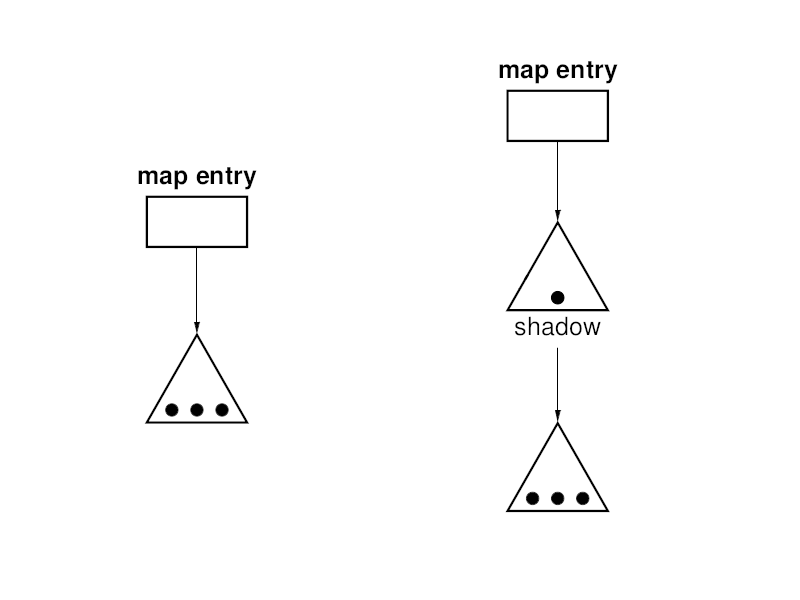
\includegraphics[scale=0.9]{copy-shadow.png}
  \caption{Creation of shadow VM object \cite{cranor}}
  \label{img:copy_shadow}
\end{figure}

We can observe that after some time there may emerge a \mintinline{c}{shadow object chains}.
The shadow objects is private for the process that owns it, therefore after the process has forked, there will possibly be
created a new shadow object that will reference the old one.
In every created shadow object in such chain there may still be some pages, that weren't modified yet and not transferred to the upper objects.
On the figure \ref{img:multiple_shadow_objs} there is an example of a simple VM object chain.
The first shadow VM object was created by a write to the private memory region by the parent process (before fork).
After forking, each process had written to some memory page and in result both processes had to create new shadow objects to hold their changes to the memory.

\begin{figure}[h]
  \centering
  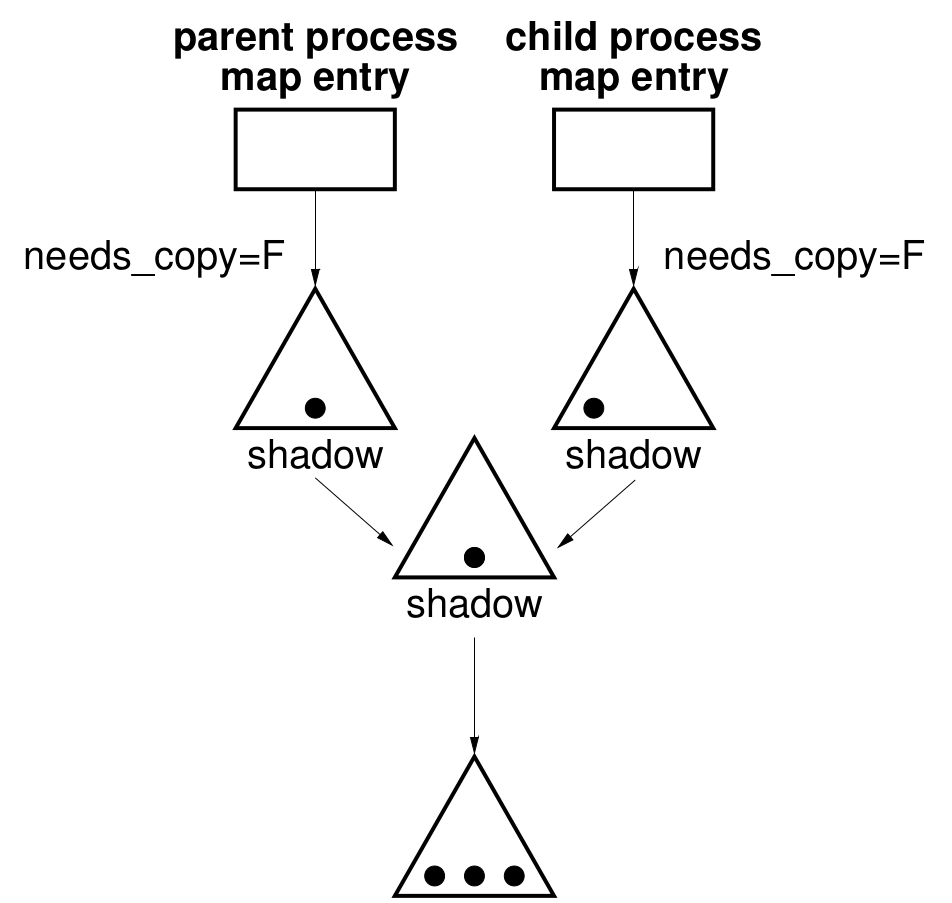
\includegraphics[scale=0.15]{multiple-shadow-objs.png}
  \caption{Two level shadow object chains \cite{cranor}}
  \label{img:multiple_shadow_objs}
\end{figure}

Because there are many levels of VM objects containing memory pages,
the page fault routine must search the entire VM object chain to locate a page in the VM~map.
This is necessary because the page may be in the lowest VM object, which is the first one created in the chain.
This process may take a long time since there is no limit to the length of the chain.

The VM object chain might be collapsed under certain circumstances.
In some cases, all pages in a shadow object have their copies in all objects above it.
To decide if an object can be removed from the chain after a page was copied to an upper VM object,
we have to pass the information about which page was copied down the chain.

The example shadow object chain that can be collapse is presented on figure \ref{img:collapse_shadow_chain}.
The only page that belongs to the object in the middle has its copy in the object above.
Such situation is usually encountered when the child process has exited and the parent is still using memory, so all of it has been copied to the upper shadow object.

\begin{figure}
  \centering
  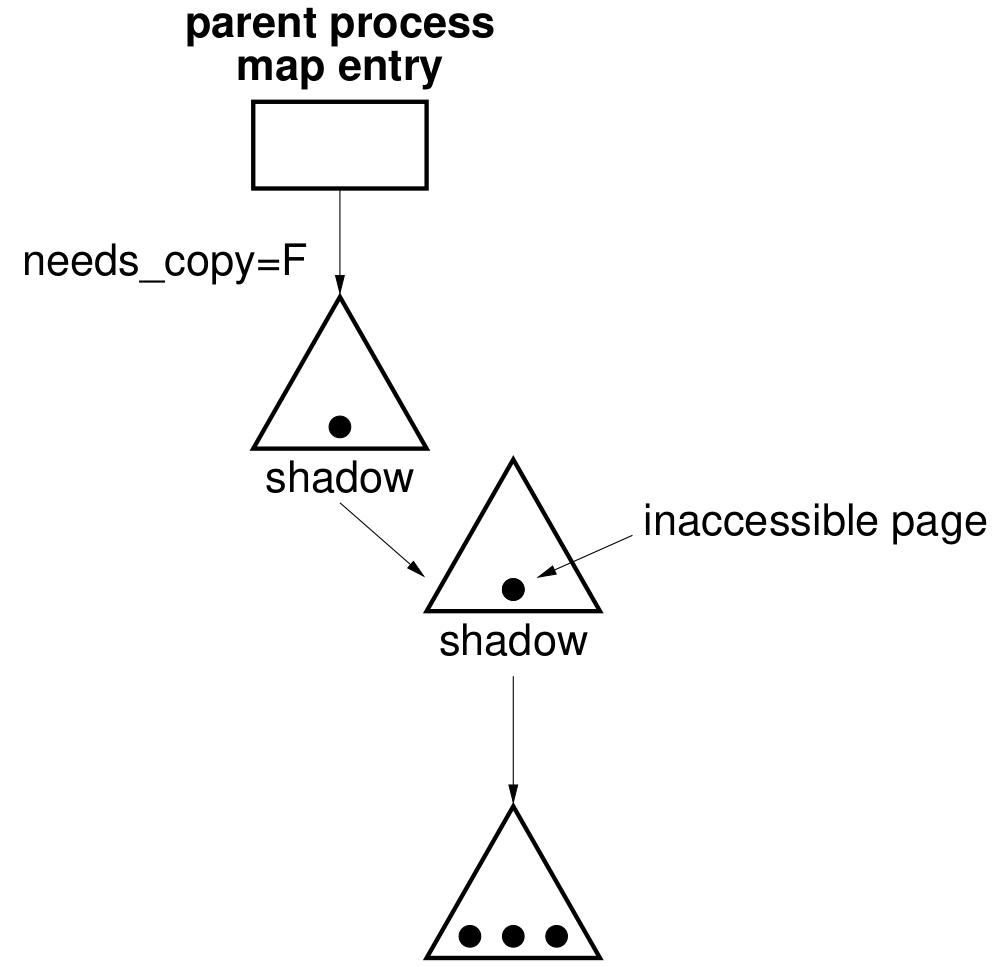
\includegraphics[scale=0.15]{collapse-shadow-chain.png}
  \caption{Shadow object chain that can be collapsed \cite{cranor}}
  \label{img:collapse_shadow_chain}
\end{figure}


\subsection{Summary of differences}

Most of the differences between UVM and BSD~VM are observed during the fork operation and the page fault routine.
These are the places which that strongly intervene with VM~map of the process.
On high level the differences are spotted due to the structure of VM~maps.
In UVM the structure is well defined and always has not more than two levels where pages could be stored.
In BSD~VM the structure might get much bigger, and harder to operate on due to possible long VM object chains.

The UVM system is also more concentrated on managing the anonymous memory.
There is more control over single anonymous pages, because they are described with separate structures designed with anonymous memory in mind.
This design makes it possible to implement new functions, that was not possible or hard to accomplish in old design.
In the original implementation of UVM there are three new operations, which were hard or impossible to implement in the old BSD~VM:

\begin{itemize}
  \item Page loan -- temporarily giving read-only access to some page to the kernel or other process.
  \item Page transfer -- transferring the page to the process VM~map from the kernel or other process.
  \item Map entry passing -- passing an VM~map entry to another process (e.g. the part of memory mapped file).
  \item Partial deallocation -- freeing the areas of anonymous memory that are no longer used (which wasn't possible in the BSD~VM).
\end{itemize}

The detailed comparison of these two implementation, as well as description of all implementation details of UVM and improvements
over the BSD~VM, is described in the Charles D. Cranor in his dissertation \cite{cranor}.

\chapter{Implementation of UVM in Mimiker}
\label{chapter:mimiker}

The practical part of this thesis is the implementation of the UVM-like virtual memory subsystem in Mimiker.
In this chapter, we will see the motivation behind this change, an overview of the system that has been implemented,
and some of the related work that has been done besides the actual implementation.

\section{The Mimiker Operating System}

Mimiker \cite{mimiker:website} is a UNIX operating system intended for research and teaching.
Its implementation is inspired by the systems from the BSD family.
Its design focuses on simplicity, as the system is used to teach students about the internals and design of the UNIX kernels.
Mimiker is still under development so there are many features that are gradually added into the kernel (one of such features is a copy-on-write support).

The Mimiker repository \cite{mimiker:sources} is used to store all the code and configuration needed to build, run, and test Mimiker.
The contents of the repository are:
\begin{itemize}
  \item Kernel code.
  \item Testing infrastructure -- both kernel and userspace tests.
  \item Userspace programs -- programs ported from the BSD systems to provide some basic user experience when launching Mimiker's shell.
  \item Scripts used to run Mimiker in Qemu emulation \cite{qemu:website}.
  \item Toolchain -- configuration and custom patches needed to prepare toolchain required to compile and simulate Mimiker.
  \item Basic documentation.
\end{itemize}

The Mimiker OS is currently ported to three different architectures: MIPS (on~Malta board), ARM (on Raspberry Pi 3) and RISCV (on HiFive Unleashed).
All these architectures support virtual memory and implement hierarchical page tables (but each of them defines different number of levels in the page table).
Later we will not talk much about the details of these architectures,
because they are not important to understand the implementation of virtual memory and copy-on-write mechanism.

\section{Motivation}

The Virtual Memory subsystem used in Mimiker was based on old BSD~VM system.
The implementation wasn't complete, there were many features missing, in particular: copy-on-write support, memory mapped files and memory swapping.
Some of such features are not implemented because there is no infrastructure to implement them
(e.g. no support for block devices or unstable VFS implementation).

Copy-on-write functionality doesn't require any additional subsystem to be enhanced beforehand.
However, after evaluating the implementation of it in current VM subsystem we have discovered that it might quickly get complicated
even if many features of virtual memory are missing.
To reduce the complexity of implemented VM system we have decided to investigate how UVM is built and replace the old VM system with it.

The integration of UVM simplified the implementation of VM system in Mimiker without losing any features.
We have made an observation that only the part responsible for anonymous memory must be implemented, because there are no other memory types supported yet.
(The first attempt to implement UVM in Mimiker failed without realizing this fact.)
We also hope that the design of UVM will help to gradually implement other VM features easily.

% \begin{itemize}
%   \item currently designed with old BSD~VM, but haven't implemented much features so far
%   \item the implementation has no CoW support
%   \item no shadow objects, no memory mapped files, no backing storage (e.g. no support for block devices)
%   \item not much to change to switch to UVM
%   \item UVM is simpler and should be easy to improve over time (with more features like mm files etc.)
%   \item Concentrate more on things that got better (not the time of operations)!
% \end{itemize}

%\comment{I want this chapter to be a guide for someone who wants to understand the Mimiker's VM design.}

\section{Implementation of UVM in Mimiker}

The current implementation of UVM in Mimiker isn't complete, because the old implementation that was replaced with UVM wasn't complete either.
However, in contrast to the previous VM subsystem, the new one will be easier to extend with new features.
Currently, only the anonymous memory mappings are available, so only the infrastructure to manage them is created so far.
The two most important features of VM system that are missing are: paging and mapping files into memory.
To get the first one we will need to extend the current implementation with support for backing storage, and to make it possible
to create mappings that reflect files memory we will need to implement UVM~objects.
Both these features will not require to change the implementation of the amaps and will require to slightly modify implementation of
anons to allow for assigning the swap number to the anon's page.
The other, more advanced features of UVM (e.g. page loanout and page transfer) are hard to evaluate now,
but they will be build upon the current implementation of amaps and anons.

\subsection{Structures}

To describe the VM~map of the process we use standard \mintinline{c}{vm_map} and \mintinline{c}{vm_map_entry} structures.
The only difference from UVM is that \mintinline{c}{vm_map_entry} structure has no reverence to the UVM~object, but only to the amap.
Both these structures, presented on listings \ref{impl:vm_map} and \ref{impl:vm_map_entry}, are defined in \mintinline{c}{sys/kern/vm_map.c} \cite{mimiker:sources}.

\begin{listing}[h]
  \begin{minted}{c}
struct vm_map {
  TAILQ_HEAD(vm_map_list, vm_map_entry) entries;
  size_t nentries;
  pmap_t *pmap;
  mtx_t mtx;
};
  \end{minted}
  \caption{VM~map structure}
  \label{impl:vm_map}
\end{listing}

\begin{listing}[h]
  \begin{minted}{c}
struct vm_map_entry {
  TAILQ_ENTRY(vm_map_entry) link;
  vm_entry_flags_t flags;
  vm_aref_t aref;
  vm_prot_t prot;
  vaddr_t start;
  vaddr_t end;
};
  \end{minted}
  \caption{VM~map entry structure}
  \label{impl:vm_map_entry}
\end{listing}

Amaps used in Mimiker are implemented using arrays.
Whey they are created, a fixed size array is allocated to be used for anons storage.
Such decision was made to make the implementation as simple as possible.
The performance problem that might occur in an array implementation is not really the issue here,
because the memory segments that appear in Mimiker are not too big and their amaps can quickly be traversed sequentially.

Amaps are referenced from \mintinline{c}{vm_map_entry} structure using a small structure aref in the same way as in UVM.
It is used to store an offset into amap, which makes it easier to split map entries without splitting or copying the amap.
The amap structure, which is presented on listing~\ref{impl:vm_amap}, is defined in \mintinline{c}{sys/kern/vm_amap.c} and the aref,
which is identical with the structure used in UVM, structure in \\ \mintinline{c}{include/sys/vm_amap.h} \cite{mimiker:sources}.

\begin{listing}[h]
  \begin{minted}{c}
  struct vm_amap {
    mtx_t mtx;             /* Amap lock. */
    size_t slots;          /* Maximum number of slots. */
    refcnt_t ref_cnt;      /* Number map entries using amap. */
    vm_anon_t **anon_list; /* Pointers of used anons. */
  };
  \end{minted}
  \caption{Amap structure}
  \label{impl:vm_amap}
\end{listing}

The other difference between UVM and its Mimiker implementation is the anon structure.
The page referenced by the anon structure can't be swapped out.
This means that the page reference will not change during the lifetime of anon, so the page for each anon can be allocated when the anon is created.
Later in this chapter we will sometimes identify anons wit pages (e.g. saying that the page is searched in the amap), because they are interrelated
and knowing a page there is exactly one anon that is referencing it.

The functions of anon could have been implemented by adding a reference counter to the \mintinline{c}{vm_page}.
However, such implementation would complicate the semantics of pages, and make it less clear how it is used.
Moreover, we hope that the UVM~objects will be implemented soon, and than having a separate structure for describing anons is mandatory.

Another difference in \mintinline{c}{vm_anon} structure, compared to the UVM, is the lack of anon lock.
Currently there is no need for such lock, because the only field that would be protected by it is the reference counter, which is currently atomic.
The anon structure, presented on listing~\ref{impl:vm_anon}, is implemented in \mintinline{c}{include/sys/vm_amap.h} \cite{mimiker:sources}.

\begin{listing}[h]
  \begin{minted}{c}
  struct vm_anon {
    refcnt_t ref_cnt; /* Number of amaps referencing this anon. */
    vm_page_t *page;  /* Page bound to the anon. */
  };
  \end{minted}
  \caption{Anon structure}
  \label{impl:vm_anon}
\end{listing}

\subsection{Operations on VM~map}

In the \mintinline{c}{sys/kern/vm_map.c} file there are defined all functions that are used by the kernel to manipulate the VM~map of the process.
Thanks to them, the implementations of individual system calls is simpler, and independent from the design of virtual memory.
These operations are also used to modify the memory map of the process in response to actions that are not directly meant to modify memory
(e.g. all operations on processes like \mintinline{c}{fork}, \mintinline{c}{execve} and \mintinline{c}{exit}).

The most important functions:

\begin{description}[style=nextline]
  \item[{\tt void vm\_map\_new(void);}]
    Initialize the new empty VM~map.
    This operation is mainly used during {\tt fork} and {\tt exec}.

  \item[{\tt int vm\_map\_insert(vm\_map\_t *map, vm\_map\_entry\_t *entry, vm\_flags\_t flags);}]
    Insert new VM~map entry into existing VM~map when it is created (e.g. when {\tt mmap} system call is used).
    By default, the VM~map entry is inserted at any address where it could fit.
    The {\tt flags} argument may be used to change that behavior.
    The flags that are passed to this function come from the {\tt mmap} argumets:
    {\tt VM\_FIXED} -- specifies that the VM~map entry must be inserted at specified addresses, and
    {\tt VM\_EXCL} -- which additionally will force unmapping of any other memory mappings that overlaps with inserted one.

  \item[{\tt int vm\_map\_entry\_resize(vm\_map\_t *map, vm\_map\_entry\_t *ent, \\vaddr\_t new\_end);}]
    This function can either extend the address range covered by given map entry or reduce it.
    The VM~map entry can be extended when the underlying amap is big enough
    (currently amaps cannot be extended, but they are created with few extra slots that can be used when entry is extended).
    When the map entry is shrunk, the pages that were previously used to store data must be unmapped.
    This function is used, for example, when the program break is moved by {\tt brk} and {\tt sbrk} system calls.

  \item[{\tt vm\_map\_entry\_t *vm\_map\_find\_entry(vm\_map\_t *vm\_map, vaddr\_t vaddr);}]
    Function that determines the VM~map entry which describes given address.
    When no map entry is describing it, {\tt NULL} value is returned.

    The lookup of the VM~map entry is very handful operation and is used by almost all functions that implement system calls actions.
    When the requested operation is served there is usually a need to find the VM~map entry specified by the address given as an argument to the system call.
    (E.g. when removing the mapping, we have to first find the VM~map entry that is representing the memory that will be removed.)

  \item[{\tt int vm\_map\_protect(vm\_map\_t *map, vaddr\_t start, vaddr\_t end, \\vm\_prot\_t prot);}]
    Change access protection for specified address range.
    If part of VM~map entry must be changed, for instance because the start address is inside the memory segment,
    then the VM~map entry is split into two individual entries, and the protection is changed only for the affected entry.
    After updating information about access protection, it must be also updated in page table.
    This function is used when the protection change is requested by the {\tt mprotect} call,
    or when the new segments with the specified protection are created during the creation of a new process during {\tt exec}.

  \item[{\tt int vm\_map\_destroy\_range(vm\_map\_t *map, vaddr\_t start, vaddr\_t end);}]
    Remove all memory segments within specified range when it is requested by {\tt munmpa} system call.
    Update page table of current process to remove address mappings that won't be valid after call to this function.
    Similarly to the previous function, if only part of VM~map entry must be destroyed then it has to be split into two parts.

  \item[{\tt void vm\_map\_delete(vm\_map\_t *vm\_map);}]
    Destroy entire VM~map of the process after it has ended its life (e.g. after calling {\tt exit} or being terminated as a result of unhandled signal).

  \item[{\tt vm\_map\_t *vm\_map\_clone(vm\_map\_t *map);}]
    Create a new VM~map during the {\tt fork}.
    Created VM~map is identical to the original one and shares all the VM~map entries with the old one.
    This function also takes care about all flags that must be set to handle properly copy-on-write entries.

  \item[{\tt int vm\_page\_fault(vm\_map\_t *map, vaddr\_t fault\_addr, \\vm\_prot\_t fault\_type);}]
    Function invoked by machine dependent code, after page fault exception was generated by MMU.
    It is responsible for finding the page that the process tried to access and inserting it into the process's page table.
    If this is impossible, because the page doesn't exit or has a different access protection than expected,
    it must return one of {\tt EACCES} or {\tt ENOMEM} to indicate the cause of the page fault.

\end{description}

The last two functions, \mintinline{c}{vm_map_clone} and \mintinline{c}{vm_page_fault}, are more complicated
and important to understand the implementation of copy-on-write.
They will be discussed in more details in following sections.

\subsection{Operations on amaps and anons}

In order to implement functions described above we need to operate on amaps and anons referenced from VM~map entries.
All essential functions used to manage amaps and anons are defined in \mintinline{c}{sys/kern/vm_amap.c}.

The most important functions:

\begin{description}[style=nextline]
  \item[{\tt vm\_aref\_t vm\_amap\_copy\_if\_needed(vm\_aref\_t aref, size\_t slots);}]
    Make copy of amap only when it is needed.
    This function is executed after {\tt VM\_ENT\_NEEDSCOPY} flag was discovered in VM~map entry holding that amap.
    Amap is actually copied when it has more than one reference.
    Such copy is done during page fault, when the new anon must be inserted into given amap.
    If amap is still shared between multiple VM~map entries, then it is automatically copied using this function to
    safely insert new anons into it.

  \item[{\tt void vm\_amap\_remove\_pages(vm\_aref\_t aref, size\_t offset, \\ size\_t n\_slots);}]
    Remove anons from specified slots in the amap (e.g. when memory segment is destroyed).
    If removed anons were referenced only by the current amap, they are freed after being removed from the amap.
    If they are referenced also by another amap, their reference count is decreased by 1.

  \item[{\tt void vm\_amap\_insert\_anon(vm\_aref\_t aref, vm\_anon\_t *anon, \\ size\_t offset);}]
    Save anon at specified offset in the amap.
    This function fails when we try to insert anon into slot where other anon is already stored.
    New anons are inserted into the amap when new anonymous memory is created or when they are copied after being shared as copy-on-write anons between multiple amaps.

  \item[{\tt vm\_anon\_t *vm\_amap\_find\_anon(vm\_aref\_t aref, size\_t offset);}]
    Check if amap has an anon at given offset and return its structure.

  \item[{\tt vm\_anon\_t *vm\_anon\_copy(vm\_anon\_t *src);}]
    Make a copy of given anon.
    The new anon is allocated and the page referenced from the original one is copied to the new one.
    Copy of the anon is needed, when anon is referenced by multiple anons but it is representing private memory.
    After copying anon, each amap that were referencing it will have its own copy of it.

\end{description}

\subsection{Cloning process VM~map}

The \mintinline{c}{vm_map_clone} function is responsible for making a copy of VM~map for the child process created during {\tt fork} operation.
Each VM~map entry that is a part of VM~map must have its copy in the new map.
Hence memory segments might be private or shared between processes, there are different rules that define how to clone them.

Whole function is organized into single loop over all VM~map entries of the old VM~map.
Each VM~map entry is examined to check its type, and using this type, proper copying function is selected.
There are two different functions:

\begin{description}[style=nextline]
  \item[\mintinline{c}{vm_map_entry_clone_shared(vm_map_t *map, vm_map_entry_t *ent);}]
    This function is used to copy a VM~map entry that describes shared memory.
    New VM~map entry is identical to the original one.
    The reference count of the amap used by both entries must be increased to record that.
    If an amap hasn't been allocated yet, it is the last time when it can be done.
    (If we don't allocate amap now, then none of the processes that is using these VM~map entries would be capable of allocating common amap.)

  \item[\mintinline{c}{vm_map_entry_clone_copy(vm_map_t *map, vm_map_entry_t *ent);}]
    This function is used to copy a VM~map entry that describes private memory.
    In this case, the amap is not copied either, but both new and original VM~map entry must be updated.
    In both entries the \mintinline{c}{VM_ENT_COW} and \mintinline{c}{VM_ENT_NEEDSCOPY} are added to flags to indicate that they represent copy-on-write segment
    and that the amap must be copied before new pages are inserted to it.
    The reference count in the amap is increased, because both entries will be using it unless it is copied.

    Additionally, page table of the parent process must be updated, to specify that the pages of the copied segment are now read-only.
    Proper access protection will be restored when they will be actually copied after first write fault.
\end{description}

After the new, copied VM~map entry is obtained, it is inserted into new VM~map.
Whole \mintinline{c}{vm_map_clone} function is presented on listing~\ref{impl:vm_map_clone}.

\begin{listing}[h]
  \begin{minted}{c}
vm_map_t *vm_map_clone(vm_map_t *map) {
  /* ... */
  vm_map_t *new_map = vm_map_new();
  vm_map_entry_t *it, *new;
  TAILQ_FOREACH (it, &map->entries, link) {
    switch (it->flags & VM_ENT_INHERIT_MASK) {
      case VM_ENT_SHARED:
        new = vm_map_entry_clone_shared(map, it);
        break;
      case VM_ENT_PRIVATE:
        new = vm_map_entry_clone_copy(map, it);
        break;
      default:
        panic("Unrecognized vm_map_entry inheritance flag: %d",
              it->flags & VM_ENT_INHERIT_MASK);
    }
    /* ... */
    TAILQ_INSERT_TAIL(&new_map->entries, new, link);
  }
  return new_map;
}
  \end{minted}
  \caption{The essential part of \mintinline{c}{vm_map_clone}}
  \label{impl:vm_map_clone}
\end{listing}

%* operation made during fork \\
%* create new vm map for the child process \\
%* each vm map entry must be either copied to new vm map or the reference is duplicated to share the entre between processes \\
%
%* the main part of the copying funciton is the loop traversing all entries of the original vm map \\
%* it is responsible for creating new vm map entry by proper function (selected based on inheritance flags) \\
%* the new entry is then inserted into the new vm map \\
%
%* this is the place where the implementation changed a lot \\
%* the vm map clone funciton is now much tidier and easier to  modify \\
%* after changing this implementation, the copy-on-write was just a matter of modifying map cone copy function \\

\subsection{Page fault handling}

Second important function of VM subsystem is handling page faults.
In Mimiker it is implemented in the \mintinline{c}{vm_page_fault} function.

The operations needed to be done during page fault are different for different types of faults.
At the beginning of the page fault routine we have to determine which scenario do we are in.
Two main scenarios are copy-on-write and non copy-on-write fault.

The copy-on-write fault happens when process is trying to write to memory which is marked as copy-on-write and still shared between two processes.
In such case, the memory must be copied.

In both cases, kernels searches for the VM~map entry that is describing the memory which is accessed by the process.
If such map entry isn't found, the access is not valid and kernel will send {\tt SIGSEGV} signal to the user process with info that
this is a map error (\mintinline{c}{SEGV_MAPERR}).
When the VM~map entry is found, then it is used to search for the page that contains faulting address.

%* another important operation in VM subsystem \\
%* invoked by machine dependent code to check if memory access that failed should in fact be successful
%
%* heavily depends on the implementation of storage for pages \\
%* how to determine cow or not cow case

\subsubsection{Standard fault}

The non-copy-on-write fault is easier to handle and is done with fewer steps:

\begin{enumerate}
  \item If amap reference doesn't exist in the VM~map entry, the amap must be created, because new page will be created and inserted into it.
  \item Page is searched in the amap (using \mintinline{c}{vm_amap_find_anon}).
  \item If page is not found, then it must be created.
  \item The found or new page must be inserted into the amap and page table.
    \begin{itemize}
      \item If VM~map entry has \mintinline{c}{VM_ENT_COW} flag set and represents segment of memory that can be written by the process,
        then the write access permission to the inserted page must be removed, to trigger copying of the page before first write to it.
    \end{itemize}
\end{enumerate}

%* amap is not present -> create \\
%* page is not found -> create \\
%* page is found -> insert \\

\subsubsection{Copy-on-write fault}

The copy-on-write fault is more complicated, and there are few things kernel must carefully do.

\begin{enumerate}
  \item If VM~map entry doesn't have an amap then create one, because we will be inserting a new anon into it.
  \item Check if amap is shared between multiple VM~map entries.
    Use \\ \mintinline{c}{vm_amap_copy_if_needed()} to obtain new \mintinline{c}{vm_aref} that will point to the correct amap
    (when amap is exclusive for the current VM~map entry, then the returned aref is identical to original one).
  \item Search for the anon in the amap.
  \item Clone the anon if it needs to be cloned.
    \begin{itemize}
      \item Check if anon's reference count is greater than 1 (if that's true, then the anon must be copied).
      \item Create a new anon with a copy of the page hold by the original anon.
      \item Replace the old anon in the amap with the reference to new one.
    \end{itemize}
  \item Insert new page table entry that describes the new page (using \mintinline{c}{pmap_enter}).
\end{enumerate}


\section{The UVM implementation process in Mimiker}

Implementing new features in the existing software is always a complicated task.
Many different parts of the codebase interact with each other and these interactions are sometimes hard to spot.
Especially when working with a huge codebase, which is the case of working on a operating system.
In Mimiker, it is common to modify many different subsystems while working on a single feature.
This is because there are many things to improve, and new or improved features help find bugs in many parts of the operating system.

\subsection{Changes prior to the UVM implementation}

Prior to the actual change in the virtual memory implementation, a few improvements were required in the old VM subsystem and other subsystems.
All these changes are aimed at improving the test infrastructure and the quality of tests of the virtual memory subsystem.
These new and modified tests helped a lot later, during the transition to the UVM.
All improvements made before this transition were implemented in the part of code that haven't been modified when implementing the UVM system.
The implementation of system calls and virtual memory tests don't require the knowledge of the structures used to store individual pages.
Because of that, the internal representation of structures which describe memory segments can be changed.

\subsubsection{New and improved system calls}

To express more operations on process memory, I had to review existing system calls to see if all the nuances of their semantics were correctly implemented.
During that process the {\tt mmap} and {\tt munmap} were improved.
{\tt mmap} system call was extended to support \mintinline{c}{VM_FIXED} and \mintinline{c}{VM_EXCL} flags.
In order to do that, the function for destroying the memory range has to be updated, to make it possible to use it in that case.
In the situation where both of these flags are set during a {\tt mmap} call, any memory that conflicts with the created memory mapping must be removed.
This change also affected the {\tt munmap} system call, because the same procedure is used to destroy memory region specified by this system call.
These changes were also aimed at being compliant with POSIX \cite{posix} standard.

The other important system call that operates on process memory is the {\tt mprotect} call.
The mechanism responsible for protecting memory from some accesses wasn't implemented at all.
Even the memory created during the {\tt exec} call wasn't protected (allowing the process to write to all memory segments, even the ones that should be read-only).

The ability to restrict memory accesses to parts of memory has been added gradually.
At first, the basic functionality was implemented in the \mintinline{c}{vm_map_protect} to allow for changing protection of whole memory segments.
At the beginning it was only used during the creation of new memory map for the process during the {\tt exec} syscall.

The next natural step was to implement a fully functional {\tt mprotect} call that would allow memory protection to be changed at any time.
The implementation of \mintinline{c}{vm_map_protect} was extended to support changing the protection of any portion of the valid memory range.
When only a part of \mintinline{c}{vm_map_entry} needs to have the access protection changed, then the entry is split into multiple parts.
The function fails, if some memory within specified range is not mapped.

After improving the system calls or creating the new ones, the tests of virtual memory must have been updated.
I have created new test cases for all new possible actions.

\begin{samepage}
Below I show pull requests that were created during that step:
\begin{itemize}
  \item \pr{1345}{[execve] Set protection bits during ELF load}
  \item \pr{1357}{Improve memory operations}
  \item \pr{1370}{Implement mprotect syscall}
  \item \pr{1383}{vm: Fix prot check in vm\_page\_fault}
\end{itemize}
\end{samepage}

\subsubsection{Improvements in signal infrastructure}

The signaling infrastructure is important for the VM memory management.
It provides a mechanism to inform the process about invalid memory operations.
The signals were already implemented, but they only provided information about the signal number and nothing more.
To provide more information, it was necessary to extend the implementation of the \mintinline{c}{sig_trap} function.
This function is responsible for recording information about the signal that will later be delivered to the process.

To provide additional information bound to the signal, the \mintinline{text}{ksiginfo_t} structure is filled in.
The structure and all functions needed to operate on it, were already implemented, but it was only used to store information about the signal number.
The important thing was to provide the additional information that will later be recorded in the \mintinline{text}{ksiginfo_t} structure.
In the case of signals used to communicate the exception caught by the kernel to the process, this information is generated in the machine-specific trap handler code.
Besides the {\tt SIGSEGV}, there are also other signals generated there ({\tt SIGBUS}, {\tt SIGFPE}, {\tt SIGILL} and {\tt SIGTRAP}).
Along with all these signals, the kernel stores more detailed information about the exception that occurred in the \mintinline{c}{ksiginfo_t} structure,
which is later translated into \mintinline{text}{siginfo_t} to be passed to the userspace signal handler.

The signals mentioned above fill in the \mintinline{text}{siginfo_t} fields with following information:
\begin{itemize}
  \item \mintinline{c}{si_addr} -- address of memory location or the instruction that triggered the signal
  \item \mintinline{c}{si_code} -- detailed information about the type of operation that caused the fault
\end{itemize}

In case of {\tt SIGSEGV} the \mintinline{c}{si_addr} points to the address that was accessed by the process and the \mintinline{c}{si_code}
tells the type of memory fault: \mintinline{c}{MAP_ERROR} -- accessed memory was unmapped, \mintinline{c}{ACC_ERR} -- memory was protected from requested access.

These improvements were introduced in pull request: \pr{1363}{Save additional information to signals}.

\subsubsection{Improvements in testing infrastructure}

The testing infrastructure is an important part of the system implementation.
It allows to quickly discover errors in newly implemented features or in the redesigned code.
With new actions available through system calls and more detailed information in signals, it was possible to implement new tests and improve the old ones.

The most important improvement was the introduction of macros that help to define parts of tests that expect to receive a signal due to a forbidden action.
Before that, it was really hard to create a test that checks if an action will fail with a given signal.
It was also impossible to test more than one such action per test, because the signal was checked after the whole test failed.

By introducing a new method of validating signals, new tests have become possible.
Now we can check if a fragment of code causes a signal, and verify that all the information delivered with it matches our expectations.
I have created a macro \mintinline{c}{EXPECT_SIGNAL} which defines which signal is expected to be received while executing instructions in the next code block.
Under the hood, this macro sets up a signal handler to record if the signal was caught, and if caught,
then saves the \mintinline{text}{siginfo_t} structure associated with it.
Immediately after using the \mintinline{c}{EXPECT_SIGNAL}, the signal handler used internally by it, must be cleared using \mintinline{c}{CLEANUP_SIGNAL}.

After successfully capturing the signal, the recorded \mintinline{text}{siginfo_t} structure should be tested for expected values.
Each signal has its own macro defined, to check appropriate fields in that structure.
In the case of {\tt SIGSEGV} the \mintinline{c}{CHECK_SIGSEGV} macro is used.
All these macros are described in the \mintinline{c}{bin/utest/util.h} header in the source code \cite{mimiker:sources}.

That new construct was added into testing infrastructure in \\
\pr{1364}{Use sigaction in all tests that need to handle SIGSEGV}.

On listings \ref{impl:segv_accerr_test} and \ref{impl:segv_maperr_test} there are two code snippets,
that test if the code inside the \mintinline{c}{EXPECT_SIGNAL} block causes the \mintinline{c}{SIGSEGV} with correct
\mintinline{c}{si_addr} and \mintinline{c}{si_code} recorded in the \mintinline{text}{siginfo_t} structure.

\begin{listing}[h]
  \begin{minted}{c}
siginfo_t si;
EXPECT_SIGNAL(SIGSEGV, &si) {
  /* The memory pointed by ptr is read protected.
   * This operation should raise SIGSEGV. */
  (void)(*ptr == 0);
}
CLEANUP_SIGNAL();
CHECK_SIGSEGV(&si, ptr, SEGV_ACCERR);
  \end{minted}
  \caption{Testing if memory read is truly forbidden.}
  \label{impl:segv_accerr_test}
\end{listing}

\begin{listing}[h]
  \begin{minted}{c}
siginfo_t si;
EXPECT_SIGNAL(SIGSEGV, &si) {
  /* The memory at addr + 0x2000 is not mapped.
   * This operation should raise SIGSEGV. */
  int data = *((volatile int *)(addr + 0x2000));
  (void)data;
}
CLEANUP_SIGNAL();
CHECK_SIGSEGV(&si, addr + 0x2000, SEGV_MAPERR);
  \end{minted}
  \caption{Test with access to unmapped memory}
  \label{impl:segv_maperr_test}
\end{listing}

\subsection{Transition to UVM}

After all preliminary work has been done we were able to change the implementation of the VM subsystem.
In fact the change was intended to be as small as possible and to simplify the whole VM implementation a lot.
It was achieved by removing two old structures (VM objects and pagers) and introducing one new structure (VM amap).
It was possible, because VM objects and pagers were used only to represent anonymous memory mappings without any additional features.
Thanks to that all required operations made on memory segments were possible to implement with just an amap.
Moreover, there was no need to implement anons at that moment, because without copy-on-write support all memory pages were eagerly copied during the fork,
so each page could be owned only by one amap at the time.
Because there wasn't introduced any new functionality, the new VM subsystem could be tested with the old tests.

The transition to UVM based virtual memory was made in \\ \pr{1379}{[vm] Simplify virtual memory subsystem}.

\subsection{Implementation of copy-on-write}

When the new VM subsystem was ready, we could finally start implementing the copy-on-write mechanism.
Thanks to the previous improvements in the VM subsystem the change was easier to create.
In this stage, the implementation of amaps was extended to make it possible to represent pages with anons which could shared between multiple amaps.

The changes that were made to create copy-on-write mechanism were done in two places: in {\tt fork} implementation and in page fault routine.
Changes made to the \mintinline{c}{vm_map_clone} function, invoked during {\tt fork}, were rather simple.
The old, eager copying of the whole VM~map was removed and instead only the flags of the VM~map entries are modified.
Whole memory is shared right after the child process is created and the private memory segments are marked as copy-on-write to be copied later.

More complicated changes were done in the page fault handler implementation in the \mintinline{c}{vm_page_fault} function.
Because now this function has to determine if the memory has to be copied, it has to handle a few new cases.
It has to carefully check the flags and reference counters of the amaps and anons to determine if they have to be copied.
Moreover, it must also adjust the permissions that are used when the found page is inserted into the process page table.

All the steps that are done in the \mintinline{c}{vm_page_fault} function:

\begin{enumerate}
  \item Create the amap if current VM~map entry doesn't have one.
  \item Search for anon in the current amap.
  \item If entry is marked as copy-on-write (call \mintinline{c}{cow_page_fault}):
    \begin{enumerate}
      \item Check if amap needs to be copied and copy it
        (it is done when \\ \mintinline{c}{VM_ENT_NEEDSCOPY} is set and amap is referenced by more than one VM~map entry).
      \item Check if anon needs to be copied and copy it (it is done when anon is referenced by multiple amaps).
    \end{enumerate}
  \item Insert anon with new (or found) page into current amap (if it isn't already there).
  \item Insert the page referenced by the found anon into the page table with correct access protection.
\end{enumerate}


%* changes in two places:
%  * fork -- rather simple change. removed copying in favour of setting few flags
%  * page fault -- some new, complicated logic
%    * few new cases (memory could be shared, partially copied or entirely copied)
%    * all of these cases must be properly identified and handled
%    * changed how amaps are copied

When working on that change, also the old tests were used unmodified because from process perspective nothing should change.
The internal design of the VM should not affect how it is exposed to user processes.

% * also the old tests were used, because processes should not notice any change, because that is only internal representation of

Copy-on-write was implemented in \pr{1392}{vm: Copy on write}.

\subsection{Further work}

The implementation described in this chapter is not complete.
Some of the features of UVM that are supported in the NetBSD system are not yet created in Mimiker.
To support them other subsystems in Mimiker must be reviewed and improved.
For instance, to implement memory mapped files we would have to improve the VFS (Virtual File System) because the main structure defined there,
\mintinline{c}{vnode_t}, will be used by UVM~objects to fetch data from the file system and place it in the process memory.
Similarly, to allow pages to be swapped to secondary storage,
we would need to ensure that we could easily interact with block devices and use them to store pages that are not currently in use.

\chapter{Performance}
\label{chapter:performance}

In this chapter we will compare two implementations of virtual memory subsystem in Mimiker, the old one and the one based on UVM.
Additionally, this chapter contains a description of a tool created to collect data for this comparison (KFT).

\section{Kernel Function Trace}

{\it Kernel Function Trace (KFT)} is a tool for obtaining trace of all functions used by the Mimiker kernel during execution.
The main idea behind KFT comes from the Linux tool {\tt ftrace} \cite{ftrace}.
However, since Mimiker is significantly different from Linux, the design of such tool had to be reinvented and adjusted for our needs.

The high-level idea behind the KFT is to record what functions were executed by the kernel while running the system.
When KFT is enabled in the build system, additional instrumentation is compiled into the Mimiker executable.
When Mimiker is launched, the information collected by the KFT can be read by the debugger.
By default, when launching Mimiker with enabled KFT, that information is saved in {\tt dump.kft} file.
Afterwards, the KFT dump must analyzed with dedicated software which is capable of parsing the KFT format used to save events recorded during the kernel execution.
I have created a Python library that can be used to design scripts to analyze KFT dumps, but it is also possible to use different language because the format
of saved data is independent from the programming language.

\subsection{The design of KFT}

\subsubsection{Function instrumentation}

To track function execution in the Mimiker kernel, additional instrumentation must be added to most kernel functions.
KFT is enabled in {\tt config.mk}, the main configuration file for the project,
by setting {\tt KFI} (Kernel Function Instrumentation) flag to {\tt ftrace} ({\tt KFI=ftrace}).
When KFT is enabled the {\tt -finstrument-functions} flag is appended to the compiler flags.
It tells the compiler to add additional code to each kernel function.
We define two functions, \mintinline{c}{__cyg_profile_func_enter} and \mintinline{c}{__cyg_profile_func_exit}, which are executed before and after each instrumented functions.
They allow us to record the time of entry and exit for each function.

By default all kernel functions are instrumented, but not all of them should.
Executing additional steps before some critical functions may drastically slow down the execution of the system or cause other more complicated problems
(e.g. indefinite recursion when instrumented function is invoked by the code added by compiler).
To exclude a function from instrumentation we must mark it with a \mintinline{c}{__no_profile} attribute.
It prevents the compiler from inserting additional code around specified function.

%* functions are instrumented because of use -finstrument-functions flag in the compiler
%* dedicated functions are created \mintinline{c}{__cyg_profile_func_enter} and \mintinline{c}{__cyg_profile_func_exit}
%* some critical functions that are executed very often are excluded from being instrumented using \mintinline{c}{__no_profile} attribute
%* The KFT instrumentation is turned on when the flag {\tt KFI} is set to {\tt ftrace}

\subsubsection{Recording events and format specification}

Each entry and exit of a function is recorded as a {\it KFT event}.
Event consists of the following information: function pc, timestamp, thread id and event type.
All these information is saved into a single 64 bit integer by applying encoding:

\begin{itemize}
  \item[\bf bit 0      ] -- Represents event type (0 for entry, 1 for exit from a function).
  \item[\bf bits 1--8  ] -- Represent the ID of thread that was executing given funciton.
  \item[\bf bits 9--42 ] -- Store the timestamp (measured in number of processor ticks from the system boot, read from hardware specific register).
  \item[\bf bits 43--63] -- Encode PC by saving the function entry address relative to \mintinline{c}{__kernel_start} symbol.
\end{itemize}

The encoded KFT event is presented on figure~\ref{fig:kft_event_encoded}.

\begin{figure}[h][h]
  \centering
  \begin{bytefield}[bitheight=\widthof{~type~}, bitwidth=0.6em, boxformatting={\centering\small}]{64}
    \bitheader[endianness=big]{64,42,9,1,0} \\
    \bitbox{21}{relative PC} & % 22
    \bitbox{33}{timestamp} & % 33
    \bitbox{8}{thread id} & % 8
    \bitbox{2}{\rotatebox{90}{type}} % 1
  \end{bytefield}
  \caption{Meaning of the bits of the encoded KFT event}
  \label{fig:kft_event_encoded}
\end{figure}

All functions that are used to create and record KFT events are defined in \mintinline{c}{sys/kern/kftrace.c}.
KFT events are saved to the global buffer which is allocated during the kernel init.
After KFT is initialized events are appended to that buffer.
When buffer is full, the \mintinline{c}{kft_flush} function is called.
The function itself does nothing but clear the buffer by setting the number of recorded events to zero.
To actually save the data gathered by KFT, we must use GDB debugger.
It stops on \mintinline{c}{kft_flush} function and copies out all data saved in the buffer, before new events are recorded.
When debugger is not attached, then all data created by KFT is discarded.

%* The KFT format is defined in \mintinline{c}{sys/kern/kftrace.c} file.
%* The two types of events are recorded: function enter and exit.
%* We also record the timestamp and the thread where the event has happened.
%* The PC (program counter) is used to record the function that has been entered or exited.
%  * It is relative to the kernel start address (to make it shorter, but still easy to decode).
%* The single event is encoded in a single 64 bit number.

\subsection{Analyzing KFT dumps}

After KFT dump is obtained from a single Mimiker run we can analyze it.
I~have created a Python library, called {\tt kftlib}\footnote{\url{https://github.com/cahirwpz/mimiker/tree/master/kftlib}},
which is capable of translating raw dump to a list of structures understood by Python.
That library may be used to implement more complicated scripts for various analysis of the dump.

\subsubsection{Details of translating KFT dump into readable format}

To correctly decode information saved in KFT dump, we first need to analyze Mimiker ELF file.
We need to extract function symbols from it and create a correspondence between function names and their addresses.
(Recall that KFT saves only an entry address of the function.)
I have used {\tt pyelftools} Python library \cite{pyelftools:sources} to access details of it.
To create meaningful representation of gathered KFT data we make few transformations of raw data:
\begin{enumerate}
  \item Decode each entry -- we need to transform single 64 bit integer to values describing single KFT event.
    We use the same scheme as presented in previous section.
    Additionally, to translate relative PC into real PC we use the location of \mintinline{c}{__kernel_start} symbol read from the ELF file.
  \item Assign events to different threads -- we use the thread number associated with an event to distribute events between threads.
  \item Calculate timestamps within threads -- for each thread we create separate timeline, which starts when the thread was created.
    We need to adjust timestamps of functions withing single thread, because they are not correct when thread was preempted by another one.
    We can observe when context switches happened (its when the thread identifier changes between two consecutive events).
    Using that information we can calculate the timestamps for events withing single thread.
\end{enumerate}

As a result of those transformations we obtain separate traces for each thread that was running during the kernel execution.
Each event contains information about its type, PC of the function and the timestamp.
In this representation, timestamp represents number of ticks that passed from the creation of the thread, but only when this thread was running.

Using such representation we can now do more transformations to get some valuable information out of it.
Examples of different information that we can extract from KFT dump:

\begin{itemize}
  \item Count how many times function was invoked by calculating number of entry events.
  \item Calculate running time of the function by determining entry and exit events and calculating the difference between their timestamps.
  \item Create call graph representing how next functions were invoked (example presented on figure~\ref{fig:call_graph}).
\end{itemize}

\begin{figure}[h]
  \centering
  \begin{minted}{text}
         time  function
          ---  ----
            0  vm_map_clone
           88  | vm_map_new
          803  | | vm_map_setup
         1062  | | *
         1149  | | pmap_new
         4868  | | *
         4954  | *
         5079  | vm_map_entry_clone_copy
         5162  | | vm_map_entry_copy
         5246  | | | vm_map_entry_alloc
         6068  | | | *
         6153  | | *
         6241  | | vm_amap_hold
         6494  | | *
         6590  | | pmap_protect
        24930  | *
               (...)
        49747  *
  \end{minted}
  \caption{Fragment of a call graph generated for \mintinline{c}{vm_map_clone} function}
  \label{fig:call_graph}
\end{figure}

I have chosen to create a python library instead of single script for analyzing KFT dumps because I think it is more flexible solution.
Every analysis, can be expressed with a single script which is easier to create, read and maintain.
At the end of this chapter, on listing~\ref{impl:kft_script}, I present an example script, which was used for generating data used in next section to create graphs.

%* analyzing kft dumps \\
%  * prepared python library that implements parsing of the dumps \\
%  * library can be used to parse the kft dump \\
%  * creates easier to process representation of all entries \\
%    * trace is split into individual threads \\
%    * timestamps are corrected (taking into account context switches) \\
%    * individual trace for each thread that was running \\
%  * using the structure created by kftlib user can write his own script \\
%    * more flexible tool
%
%* explain the timestamps (why we don't care about exact time, only the number of ticks)

\subsection{Performance of the new VM subsystem}

The performance of the new UVM subsystem with implemented copy-on-write feature is measured on the Mimiker's tests execution.
I am comparing two versions of Mimiker:

\begin{description}
  \item[New]
    The newest version of Mimiker with all new features and optimizations.
    \footnote{At the time of writing this thesis the latest commit is
    \href{https://github.com/cahirwpz/mimiker/commit/3dffeafce8dbba33741505163d7856dbc0f1dd36}{\tt 3dffeafce8}}
  \item[Old]
    The version with old implementation of virtual memory subsystem.
    It is tracked by the branch {\tt old-vm-master}\footnote{\url{https://github.com/cahirwpz/mimiker/tree/old-vm-master}}.
    To accurately compare those two versions, all changes made to the kernel and not related to the transition to UVM were applied to the old version too.
\end{description}

Below I show a few histograms and all of them show the same data for different functions.
There are two types of plots that we will see there:
\begin{itemize}
  \item Bar plots -- they present the difference in the number of function calls for given functions.
  \item Histograms -- they present a distribution of running times for given functions.
    On the x-axis there is an execution time and on the y-axis there is a number of invocations that ran for a given time.
\end{itemize}

\subsubsection{Comparison between old VM and UVM with copy-on-write}

One of the main goals of this thesis was to implement copy-on-write mechanism which reduces number of page copies.
Thanks to the new virtual memory mechanism we copy only pages that really needs to be duplicated.
On figure~\ref{plot:pmap_copy_page} we can see that \mintinline{c}{pmap_copy_page} function, which is used by the kernel
to make a copy of given page, is used almost 13 times less than before.

\begin{figure}[h]
  \centering
  \createbar{9652}{700}
  \caption{The number of \mintinline{c}{pmap_copy_page} invocations}
  \label{plot:pmap_copy_page}
\end{figure}

The other results, which emerges from the fact that we now make much less copies of pages, is that we also use less pages in total.
On the figure~\ref{plot:vm_page_alloc} we can see, that we use about 5 times less pages than previously.
In Mimiker all pages have size 4 KB, hence the space saved thanks to copy-on-write is about 4 MB.

\begin{figure}[h]
  \centering
  \createbar{10822}{1870}
  \caption{\mintinline{c}{vm_page_alloc}}
  \label{plot:vm_page_alloc}
\end{figure}

Because all page copies are now performed on demand and not in the \mintinline{c}{vm_map_clone}, that function is much faster now.
All invocations of \mintinline{c}{vm_map_clone} are now almost 2 times faster than all invocations of the same function in the old implementation.
The comparison of two implementations of this function is presented on histogram on figure~\ref{histogram:vm_map_clone}.
Those results show, that after {\tt fork} both parent and child processes will start executing faster,
because they don't have to wait until all parent memory is duplicated.

\begin{figure}[h]
  \centering
  \createhist{plots/data-old/vm_map_clone.data}{plots/data-new/vm_map_clone.data}{xmin=0, xmax=130000, legend style={at={(0.02,0.89)},anchor=west}}
  \caption{\mintinline{c}{vm_map_clone}}
  \label{histogram:vm_map_clone}
\end{figure}

The other important function that we care about is \mintinline{c}{vm_page_fault}.
Execution time of page fault handling routine as well as the number of page faults has increased.
Both these results are expected.
The time has increased, because page copies are now performed here instead of during fork.
The number of page faults has increased, because copy-on-write segments generate now additional page faults.
Parent process will generate one additional page fault when it will try to write to copy-on-write segment.
Child process may generate two page faults on the same memory when it accesses such segment first with read operation and later with write operation.
In the original implementation child generated only one page fault, and parent didn't generate any page fault at all,
because its memory was always present and ready to be access with any allowed operation.

On the histogram on figure~\ref{histogram:vm_page_fault} we can observe one more thing.
Now, the function execution times vary more.
It's happening because now we have more things to do when page fault is handled (e.g. copy an amap or anon).
The optimistic result is that still most of page faults are short.

\begin{figure}[h]
  \centering
  \createhist{plots/data-old/vm_page_fault.data}{plots/data-new/vm_page_fault.data}{xmin=0, xmax=47000}
  \caption{\mintinline{c}{vm_page_fault}}
  \label{histogram:vm_page_fault}
\end{figure}

One more reason, why page faults are now slower is the fact that we need to allocate additional structures, when copying page from copy-on-write segment.
The comparison of functions used to allocate VM objects and amaps is presented on figure~\ref{histogram:alloc}.
We can see that allocation of amaps takes more time.
That's because, they require additional array to store references to anon structures.
VM objects didn't require allocation of additional space, because they used linked list structure to store their pages.
On figure~\ref{histogram:kmalloc} we can see, that the increase in \mintinline{c}{kmalloc} function usage matches the usage of amaps allocation function.
This function is internally used by amaps to allocate memory for list of anons.

To explain why some calls to \mintinline{c}{vm_amap_alloc} take so much time we have to look what function are executed during those calls.
Those are cases, when \mintinline{c}{kmalloc} runs out of preallocated memory and have to alloc new memory pool for later allocations.
This operation takes a lot of time because it allocates a large amount of memory in advance to make later allocations faster.

\begin{figure}[h]
  \begin{subfigure}{0.45\textwidth}
    \centering
    \createhist{plots/data-old/vm_object_alloc.data}{plots/data-new/vm_amap_alloc.data}{xmin=-100, xmax=22000}
    \caption{\mintinline{c}{vm_object_alloc} vs \mintinline{c}{vm_amap_alloc}}
    \label{histogram:alloc}
  \end{subfigure}
  \hfill
  \begin{subfigure}{0.45\textwidth}
    \centering
    \createhist{plots/data-old/kmalloc.data}{plots/data-new/kmalloc.data}{xmin=-100, xmax=22000}
    \caption{\mintinline{c}{kmalloc}}
    \label{histogram:kmalloc}
  \end{subfigure}
  \caption{Additional allocations}
\end{figure}

We can think about optimizing it, but we can't use simple linked list as before.
Because pages are shared between multiple amaps we would need to store them on multiple linked lists.
For each such list, a pointer to next list item must be saved somewhere.
This means, we would have to allocate some amount of memory for such pointers in each anon, but this is wasteful,
because we don't know which anons will be shared and by how many amaps.

If we had decided that we still want to use VM objects to represent memory, we would have also allocate more memory.
Instead of allocating memory for page list, we would use more VM objects (where some of them would be shadow VM objects).
In contrast, due to reduction of number of pages that needs to be copied during process lifetime, we allocate less amaps,
because some of them are shared between multiple VM~map entries (but we can't accurately compare it with the number of allocated VM objects,
because we have no implementation of copy-on-write which is using old VM infrastructure).


The new design of structures used to store pages has also good results.
On figure~\ref{histogram:find_page} we can see a comparison of functions that are used to search for pages in VM objects and in amaps.
We can see, that all execution of \mintinline{c}{vm_amap_find_anon} takes roughly the same time.
It happens because we already know the offset of searched page and the anon lookup is a constant operation in amap.
In VM objects, we had to traverse the linked list of pages to find the one we were looking for.
The number of page lookups is greater, because page is searched during page fault, which has increased the number of occurrences.

\begin{figure}[h]
  \centering
  \createhist{plots/data-old/vm_object_find_page.data}{plots/data-new/vm_amap_find_anon.data}{xmin=100, xmax=300}
  \caption{old \mintinline{c}{vm_object_find_page} vs new \mintinline{c}{vm_amap_find_anon}}
  \label{histogram:find_page}
\end{figure}

The last function in this comparison is \mintinline{c}{pmap_protect}.
We started using it and we can clearly see that it is used a lot more than in the old VM subsystem.
Previously it was only used during {\tt exec} to assign proper memory protection flags to segments loaded from executable file.
Now \mintinline{c}{pmap_protect} is also used during {\tt fork} to protect copy-on-write segments from writing, until written memory is copied.
We expected that the number of operations that require changing memory protection will increase.
On the figure~\ref{histogram:pmap_protect} we can also see that there are various different calls to \mintinline{c}{pmap_protect} function
because memory regions of different size are protected.

\begin{figure}[h]
  \centering
  \createhist{plots/data-old/pmap_protect.data}{plots/data-new/pmap_protect.data}{}
  \caption{\mintinline{c}{pmap_protect}}
  \label{histogram:pmap_protect}
\end{figure}

Additional analysis shows that the \mintinline{c}{pmap_protect} is the main cause of additional time spent in the VM functions.
If we calculate total time of \mintinline{c}{vm_map_clone} and \mintinline{c}{vm_page_fault} in both old and new implementations we can see that
the difference between them is roughly the total time of \mintinline{c}{pmap_protect} function.
Total running times of mentioned functions are listed in the table~\ref{table:fn_times}.

\begin{table}[h]
  \centering
  \begin{tabular}{ |l|r|r|r|r| }
   \hline
    Function name & Count & Total time \\
   \hline
   \hline
    \mintinline{c}{vm_map_clone} (old) & 146 & 16508512 \\
    \mintinline{c}{vm_map_clone} (new) & 146 &  9356264 \\
   \hline
   \hline
    \mintinline{c}{vm_page_fault} (old) & 2958 & 12695736 \\
    \mintinline{c}{vm_page_fault} (new) & 3668 & 26167512 \\
   \hline
   \hline
    \mintinline{c}{pmap_protect} (old) &   30 &   48360 \\
    \mintinline{c}{pmap_protect} (new) & 1041 & 6972618 \\
   \hline
  \end{tabular}
  \caption{Comparison of total execution time of VM functions}
  \label{table:fn_times}
\end{table}

\subsubsection{Summary of performance analysis}

The above performance comparisons show two things: the new implementation is more effective in terms of memory usage,
but its slightly slower than the previous solution.
The first outcome is expected, because that is the reason why we wanted to implement copy-on-write mechanism in Mimiker.
The second result is in fact hard to analyze.
To be 100\% sure which implementation of VM is better in terms of time consumption we should have compared two versions of VM with the same set of features.
In our case it isn't possible, because the old version doesn't have implemented a copy-on-write mechanism.
However, the performance analysis described in \cite{cranor} shows that the design used by UVM is more effective than the traditional one previously used in NetBSD.

The other reason why this performance improvement cannot be directly measured in Mimiker, is that there are still left some features to implement.
The VM subsystem is still simplified in comparison to fully functioning UVM implementation.
The new design will help with effective implementation of other parts of the VM such as memory mapped files and paging mechanism.

\section{Generating data for analysis}

To generated the data for the performance analysis we have to obtain the Mimiker source code.
Whole Mimiker project is maintained in a single repository on GitHub \cite{mimiker:sources}.
It contains: the source code, tests, userspace programs, scripts to build and run Mimiker simulation, toolchain needed to develop Mimiker
and a documentation.

\subsection{Toolchain installation}

To develop and use Mimiker we need to install a custom toolchain.
All sources needed to compile custom programs are included in Mimiker's repository in {\tt toolchain} directory.
Installation steps and other helpful information about Mimiker development can be found on the project wiki page \cite{mimiker:wiki}.

\subsection{Building Mimiker}

Right before building Mimiker we have to adjust the configuration file to enable KFT instrumentation.
Configuration is read from {\tt config.mk} file in Mimiker's root directory.
To enable KFT we need to set {\tt KFI} flag ({\it Kernel Function Instrumentation}) to {\tt ftrace}.

After adjusting configuration we can finally build OS by running {\tt make} command.
The most important file produced during build, in context of later analysis, is the Mimiker binary present at path {\tt sys/mimiker.elf}.

\subsection{Running and collecting KFT dump}

After successful build we can finally start a Mimiker simulation in Qemu.
We use {\tt launch} script to run Mimiker and specify configuration options to adjust the running environment and specify program that will be executed.
In our case the command is: {\tt ./launch -b rpi3 -d -k utest=all}.

\begin{itemize}
  \item {\tt -b rpi3} -- specifies the board that the Mimiker was build for ({\tt rpi3} is the default board)
  \item {\tt -d} -- starts debugging session
  \item {\tt -k} -- enables support for collecting KFT dumps by the debugger
  \item {\tt utest=all} -- specifies that we want to run all user space tests
\end{itemize}

After tests have finished we have to manually close the debugging window that was opened (e.g. by hitting {\tt Ctrl+B D} sequence).
KFT dump is saved to {\tt dump.kft} file on a host machine.

\subsection{Analyzing KFT dump}

Finally, we can use a Python script to generate data that is easier to analyze: call graphs of given functions and data needed to create plots.
To use {\tt kftlib} we have to install it using \mintinline{sh}{pip install ./kftlib} command in the Mimiker directory.
Example script that can be used to generate date for plots in previous section is presented on listing~\ref{impl:kft_script}.
More advanced scripts as well as the details of {\tt kftlib} can be seen in the \pr{1418}{KFT python lib}.

\begin{listing}[h]
\begin{minted}{python}
#!/usr/bin/env python3
import kftlib
import statistics
import os

def get_fn_times(events, elf, functions, out):
    fn_pcs = list(map(lambda fn: elf.fun2pc.get(fn), functions))
    fn_times = kftlib.get_functions_times(events, fn_pcs)
    os.makedirs(out, exist_ok=True)

    print(f"{'function':>13}: {'count':>5} {'avg time':>8}")

    for fn, pc in zip(functions, fn_pcs):
        if pc and pc in fn_times:
            # Print short summary
            avg_time = statistics.mean(fn_times[pc])
            count = len(fn_times[pc])
            print(f"{fn:>13}: {count:>5} {avg_time:>8.0f}")
            # Dump all invocations to file
            with open(f"{out}/{fn}.data", "w") as f:
                f.write("\n".join(str(t) for t in fn_times[pc]) + '\n')

def main():
    functions = [
        "vm_amap_find_anon", "vm_object_find_page", "vm_page_fault",
        "pmap_protect", "pmap_copy_page", "vm_page_alloc",
        "vm_map_clone", "vm_amap_alloc", "vm_object_alloc",
    ]
    input = [
        ("new.elf", "new.kft", "new-data"),
        ("old.elf", "old.kft", "old-data"),
    ]
    for elf_p, kft_p, out_dir in input:
        elf = kftlib.Elf.inspect_elf_file(elf_p)
        events = kftlib.inspect_kft_file(kft_p, elf)
        get_fn_times(events, elf, functions, out_dir)

main()
    \end{minted}
  \caption{Python script used to generate data for graphs in previous section}
  \label{impl:kft_script}
\end{listing}


\chapter{Conclusion}
\label{chapter:conclusion}

In this thesis I have presented the design of Virtual Memory subsystem in a UNIX system.
In particular we have seen the details of the part responsible for managing the processes memory.
Moreover, we have seen the real implementation of the UVM virtual memory subsystem with the copy-on-write mechanism in the Mimiker OS.
All changes to Mimiker, descibed in this thesis, are alread merged to the {\tt master} branch in the project repository, hence every user of the Mimiker OS is now using the new implementation of Virtual Memory.

\section{Contributions}

In previous chapters we have seen the new features added to the Mimiker while working on this thesis.
The main goal was the effective implementation of copy-on-write mechanism.
The one created there has improved the performance of the system as expected.
The number of page copies has been reduced and the kernel spends less time during a {\tt fork} system call thanks to that improvement.

Additionally, in order to make the process of implementing copy-on-write mechanism easier, I have reworked the implementation of the virtual memory map structures.
Their new design, based on the UVM, is more modular, because of different structures used to describe different types of memory.
It not only made the implementation of copy-on-write simpler, but will also help with implementing other features of virtual memory subsystem in the future.

Other changes, also in subsystems different from the VM, has improved the overall experience while developing Mimiker.
The new information associated with signals has created new possibilities while designing user space tests that weren't possible before.
In particular, the tests used to verify correctness of the VM subsystem has been improved the most.
They were extensively used while working on new VM design.

The last contribution to the Mimiker OS is the Kernel Function Trace utility.
It was used to check if the implementation introduced earlier behaves as expected.
Additionally, it helped with finding optimizations in the implementation of the virtual memory subsystem.
For example, the \mintinline{c}{pmap_protect} function was optimized to operate well on large memory regions
(before it was implemented to work effectively on on single page regions).

Because the KFT is split into two independent parts: kernel part and library for analysis,
it may be used in the future for similar performance analysis for other parts of the kernel.
Because the Python library translates KFT dump into format that is easy to manage within Python,
it can be used to implement any kind of analysis on the data gathered during Mimiker run.

\section{Future work}

As mentioned earlier, the new design will allow for gradual and simpler implementation of next features of the VM subsystem.
Two of them, memory mapped files and paging, are the most important ones.
Memory mapped files will use the UVM~objects as a structure to describe the memory that will reflect the contents of a file.
However, they require also some work in the scope of Virtual File System in order to manage the files that are accessed via file system.
The VFS implementation in Mimiker needs to be revisited and improved to make it possible to interact with other subsystems.

The paging mechanism is also the one that should be possible to add in the future.
It will implement the interaction between virtual memory and devices used to store data.
The infrastructure needed to operate on block devices, that are used to store blocks of data, needs to be created in Mimiker.
Once the paging mechanism is implemented, it will allow to swap out pages from main memory to the backing storage.

There are also other features that can be later added, but are not essential in the Mimiker at the moment.
For instance, the additional UVM mechanisms that were mentioned in one of the previous chapters (page loan, page transfer and map entry passing).
They are not essential, because they solve problems that aren't currently experienced in the Mimiker, because they are used during operations that
are impossible or not extensively used in the Mimiker (e.g. fetching large chunks of data from the internet) .


\bibliographystyle{unsrt}
\bibliography{bibliography}

\end{document}
